\documentclass[11pt]{article}

\usepackage{graphicx}
\graphicspath{{Figures/}{../}{../figs/}}

\usepackage{gensymb}
\usepackage{mathtools}
\usepackage{amssymb}
\usepackage{amsmath}

\usepackage{xcolor}
\usepackage{subfigure}

\usepackage[font=footnotesize,labelfont=bf]{caption}

\usepackage[T1]{fontenc}

\renewcommand{\rmdefault}{ppl}
\renewcommand{\sfdefault}{phv}
\renewcommand{\ttdefault}{pcr}
\renewcommand{\familydefault}{\sfdefault}

\usepackage{fancyhdr}
\fancypagestyle{plain}{
  \fancyhf{}
  \fancyhead[R]{\thepage}
}
\renewcommand{\headrulewidth}{0pt}

\usepackage{geometry}
\geometry{letterpaper}
\geometry{margin=2cm}
\renewcommand{\topfraction}{0.95}
\renewcommand{\bottomfraction}{0.9}
\renewcommand{\textfraction}{0.02}
\renewcommand{\floatpagefraction}{0.5}
\usepackage{placeins}

\renewcommand{\baselinestretch}{1.25}
\setlength{\parindent}{0in}
\setlength{\parskip}{0.1in}

\usepackage{url}
\usepackage{microtype}
\setlength{\emergencystretch}{2em}

\begin{document}

\section*{\LARGE  Invariance and selectivity to spatial variables in deep neural networks and the brain }

Margaret C Von Ebers\textsuperscript{1,3,4} and Xue-Xin Wei\textsuperscript{1,2,3,4,5}

1) Department of Neuroscience, The University of Texas at Austin\\
2) Department of Psychology, The University of Texas at Austin\\
3) Center for Perceptual Systems, The University of Texas at Austin\\
4) Center for Theoretical and Computational Neuroscience, The University of Texas at Austin\\
5) Center for Learning and Memory, The University of Texas at Austin

\section*{Abstract}
Although it is generally thought that the formation of cognitive maps requires the brain to integrate self-movement (i.e., path integration), recent studies challenge this view by showing the existence of spatial selectivity in deep networks trained with vision inputs alone.
Because these studies only examined neuronal selectivity to individual spatial variables (e.g., location, head direction), without characterizing their joint tuning,
it remains possible that the ways in which space is encoded in the brain and in these models are substantially different.
We develop an analysis framework for the joint tuning of neurons to multiple spatial variables and apply it to the rodent brain and to recently proposed vision-based deep networks. Neurons in the brain and in the models show qualitatively different selectivity and invariance to location and head direction. Our results demonstrate the importance of studying joint tuning properties in understanding neural codes.

\newpage
\section{Introduction}

Examining the tuning property of individual neurons is a basic approach for studying the neural code~\cite{Hubel1959,o1971,Hafting2005,Deangelis1991,decharms2000neural,Stensola2012,Kriegeskorte2021}. Over the past few decades, neuroscientists have characterized the tuning properties of neurons to behavioral variables in many brain regions~(e.g., \cite{Hafting2005,Deangelis1991,decharms2000neural,Stensola2012,Taube1990}).
In the hippocampus and related brain areas (e.g., entorhinal cortex and parahippocampus), neurons selective to various spatial variables (e.g., location, head direction, speed) have been discovered~\cite{o1971,o1978,Hafting2005,Stensola2012,Kropff2015speed,Taube1990}. Earlier studies focused mainly on the selectivity to one stimulus variable (e.g., visual orientation, location, or head direction). More recent studies also examined the selectivity of neurons to multiple stimulus dimensions individually. If a neuron is selective to multiple variables, the neuron is considered to exhibit conjunctive tuning~\cite{Sargolini2006conjunctive} or mixed selectivity~\cite{Rigotti2013,Fusi2016neurons,Hardcastle2017multiplexed}.

A large body of work has investigated how the brain constructs spatial maps of the environment. This question is relevant both for understanding how the brain supports navigation~\cite{Mcnaughton2006} and for building embodied intelligent agents~\cite{Cadena2017}.
It is generally believed that the brain integrates self-movement signals (i.e., velocity input and head rotation) to generate such maps~\cite{Mcnaughton2006} (the path integration hypothesis~\cite{Darwin1873}). Other sensory inputs, such as visual landmarks and boundaries, are thought to recalibrate the cognitive map~\cite{Hardcastle2015environmental,Zhang1996}. Recurrent neural network models, either hand-crafted~\cite{Samsonovich1997,Zhang1996,Burak2009} or optimized for navigation tasks~\cite{Cueva2018,Banino2018,Sorscher2020,Cueva2020,Gao2021}, have been developed to model place cells, head direction cells, and grid cells.
Recent studies challenged this view. In deep neural network models trained to solve purely visual tasks, many network units exhibit spatial selectivity that resembles that observed in the rodent hippocampus~\cite{Gornet2024automated,Luo2024}.
When comparing the brain and the models, these studies examined the marginal tuning of each neuron to individual stimulus variables, one at a time. Recovering joint tuning from marginal curves requires additional assumptions about response structure and stimulus sampling; marginal curves alone can misrepresent how a neuron depends on each variable.

Here we directly analyze the \textit{joint tuning} of individual neurons to multiple stimulus variables \textit{simultaneously}.
We first show that the tuning curve for one variable at a time can miss important information about the tuning properties.
We then develop an analysis framework for the selectivity and invariance of the neuronal response when multiple stimulus variables are considered together. Applying this framework to rodent spatial navigation circuits and to recently proposed deep neural network models of these circuits yields three main findings. First,
hippocampal CA1 neurons show greater tuning-shape dependence on location than on head direction, whereas postsubicular head direction cells show the converse preference. Second, units in deep neural network models trained to perform vision tasks~\cite{Luo2024,Gornet2024automated} exhibit entangled tuning for location and head direction, and are therefore markedly distinct from place cells and head direction cells in rodents.
Third, rodent head direction cells show much stronger tuning-shape dependence on head direction than on movement direction, and decode head direction much more accurately.
Using spatial navigation as an example, our results demonstrate the importance of analyzing the joint tuning of neurons in order to understand the structure of the representation in the brain and in deep neural networks.

\begin{figure}[p]
\centering
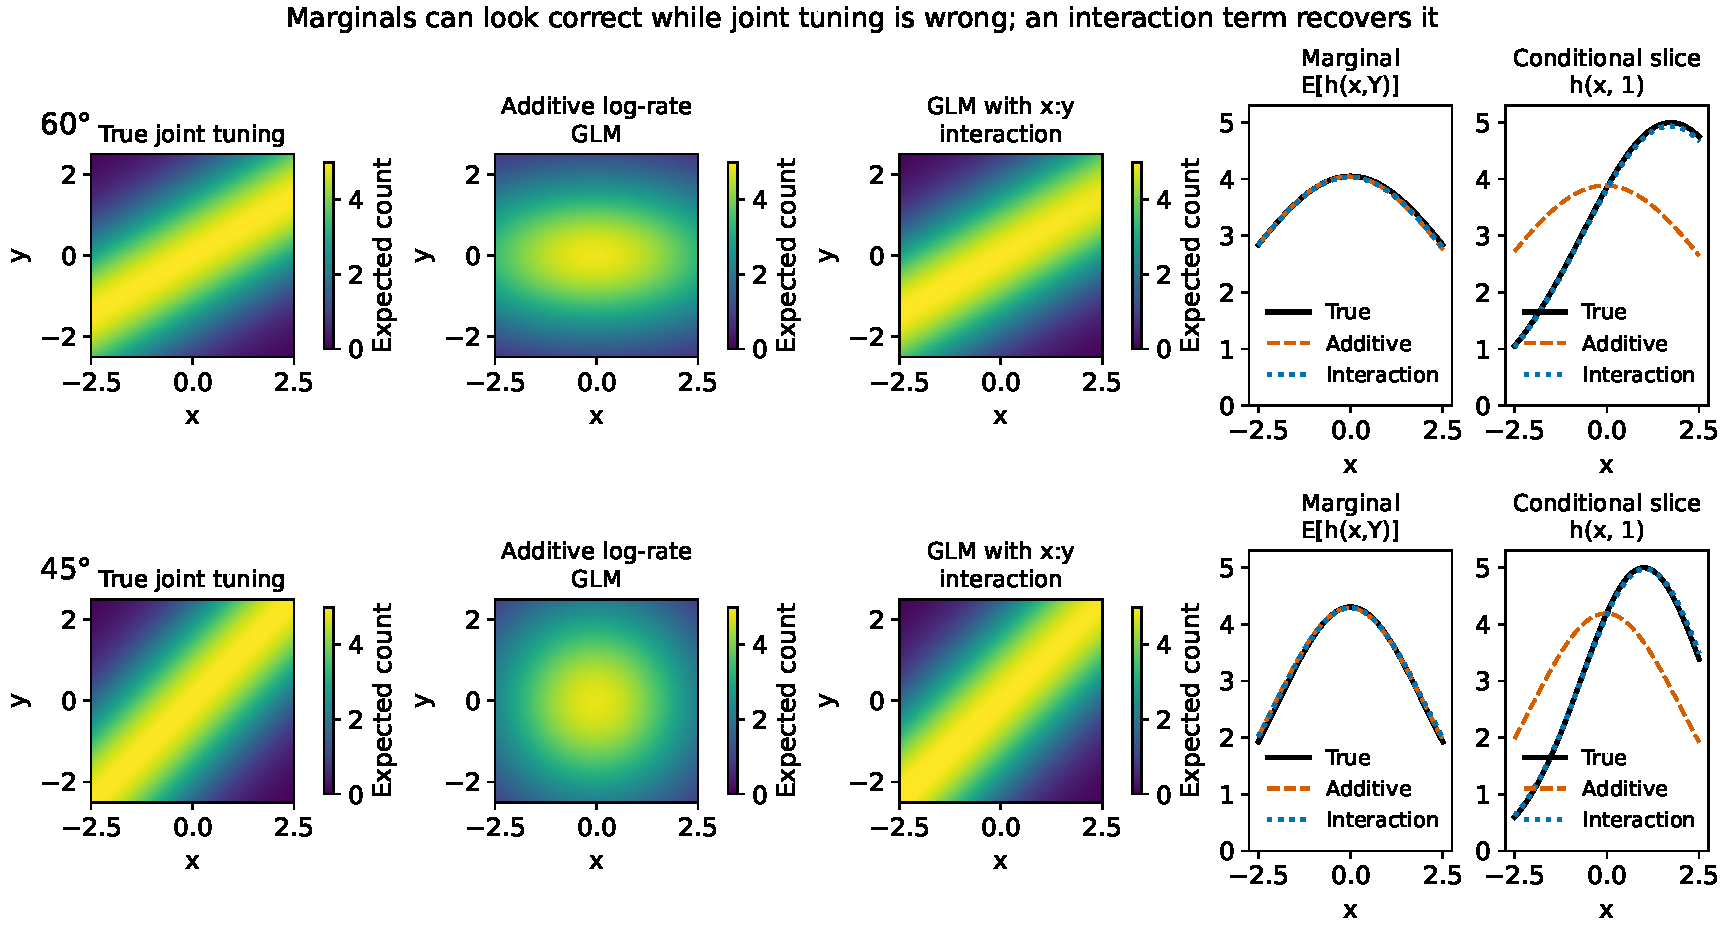
\includegraphics[width=.98\textwidth]{final_figures/glm_corrected.pdf}
\caption{\textbf{An additive log-rate GLM misses an interaction that is recovered by an interaction GLM.} Rows show Gaussian-ridge tuning at $60\degree$ and $45\degree$. Columns show the true joint tuning, the fitted additive model, the model including $xy$, the marginal response averaged over the actual stimulus distribution, and a conditional slice at $y=1$. Both stimuli are independent standard-normal variables. The additive model approximates the marginal but misses the conditional response; the interaction model recovers both.}
\label{fig:glm}
\end{figure}

\section{Results}

\subsection{Marginal tuning curves are insufficient to capture the joint tuning}

When only one stimulus variable (denoted $x$, such as the head direction of the animal) is considered, the tuning property of a neuron can be described by its tuning curve $f(x)$, which quantifies how the firing rate of the neuron varies with the stimulus variable.
Suppose that another stimulus variable $y$ is also of interest (e.g., the movement direction of the animal), and that our goal is to understand whether this neuron is selective to both $x$ and $y$. The standard approach is to examine the marginal tuning curves $f(x)$ and $g(y)$ separately to see whether one or both exhibit strong selectivity. If $f(x)$ is a narrow Gaussian function and $g(y)$ is flat, it is tempting to conclude that the neuron is selective to $x$ and invariant to $y$. However, this analysis of the marginal tuning curves can misrepresent the joint tuning to the two variables.

Fig.~\ref{fig:glm} illustrates this limitation with two neurons whose joint tuning contains an interaction between $x$ and $y$. A Poisson GLM with separate quadratic terms for $x$ and $y$ approximates the marginal tuning but misses the orientation of the joint tuning and its conditional slices. Adding an $xy$ interaction recovers these features and improves held-out likelihood. The marginals in these examples are not flat: the limitation is that matching them does not recover the interaction.

With an exponential link, additive functions of separate variables imply multiplicatively separable joint tuning. This restriction applies to an additive log-rate GLM, not to GLMs in general~\cite{Pillow2008spatio,Hardcastle2017multiplexed}. Explicit interaction terms relax the restriction. Direct analysis of joint tuning provides another way to examine these interactions.

\begin{figure}[htbp]
\centering
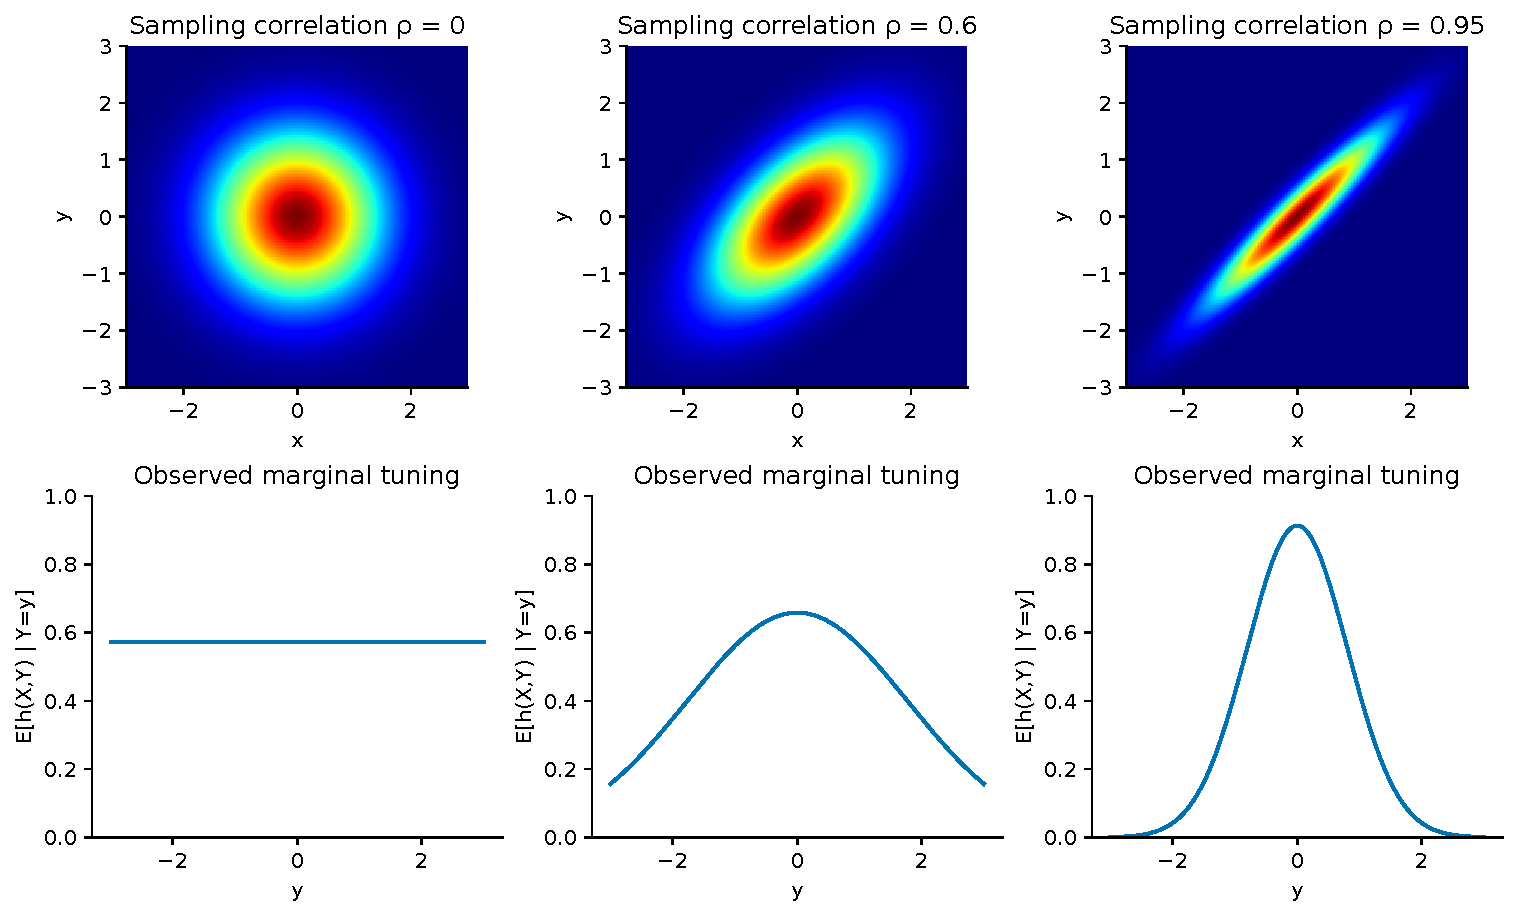
\includegraphics[width=0.9\textwidth]{final_figures/marginal_confound.pdf}
\caption{\textbf{Correlated stimulus sampling produces apparent tuning to an irrelevant variable.} The response $h(x,y)=\exp[-x^2/(2\sigma^2)]$, with $\sigma=0.7$, depends only on $x$. Top: bivariate standard-normal sampling distributions with correlations $0$, $0.6$, and $0.95$. Bottom: the analytically averaged response conditioned on $y$. Apparent tuning to $y$ increases with sampling correlation despite the response being invariant to $y$.}
\label{fig:fig1}
\end{figure}

Correlated sampling of the stimuli further complicates the interpretation of marginal tuning curves. Correlated stimulus variables are common. In spatial navigation, one notable example is the animal's head direction and movement direction~\cite{Raudies2015head}; another is time and distance traveled when the animal runs on a linear track. Suppose that a neuron is selective to $x$ and completely invariant to $y$ (Fig.~\ref{fig:fig1}). Because of the correlation in stimulus sampling, the marginal tuning curve for $y$ still shows substantial selectivity (see Methods). Relying on the marginal tuning curves alone, we would incorrectly conclude that the neuron is tuned to $y$, although its response is completely invariant to $y$. Analyzing the joint tuning directly avoids this error.

\subsection{A method for analyzing the invariance and selectivity of neurons}

The results above show that, when analyzing the selectivity and invariance of neural responses, it is necessary to examine the joint tuning beyond the marginal tuning curves. A simple way to assess whether the response is invariant to a stimulus variable $x$ is to vary $x$ and examine the tuning to the remaining variables. With two variables, this amounts to examining the tuning curve for $y$ \textit{conditioned on} different values of $x$.
If the tuning curve for $y$ does not change with $x$, the response is invariant to $x$. We distinguish this full response invariance from tuning-shape invariance: a curve can preserve its shape while its gain or baseline changes. The correlation-based statistic below quantifies the latter distinction.

\begin{figure}[h!]
    \centering
    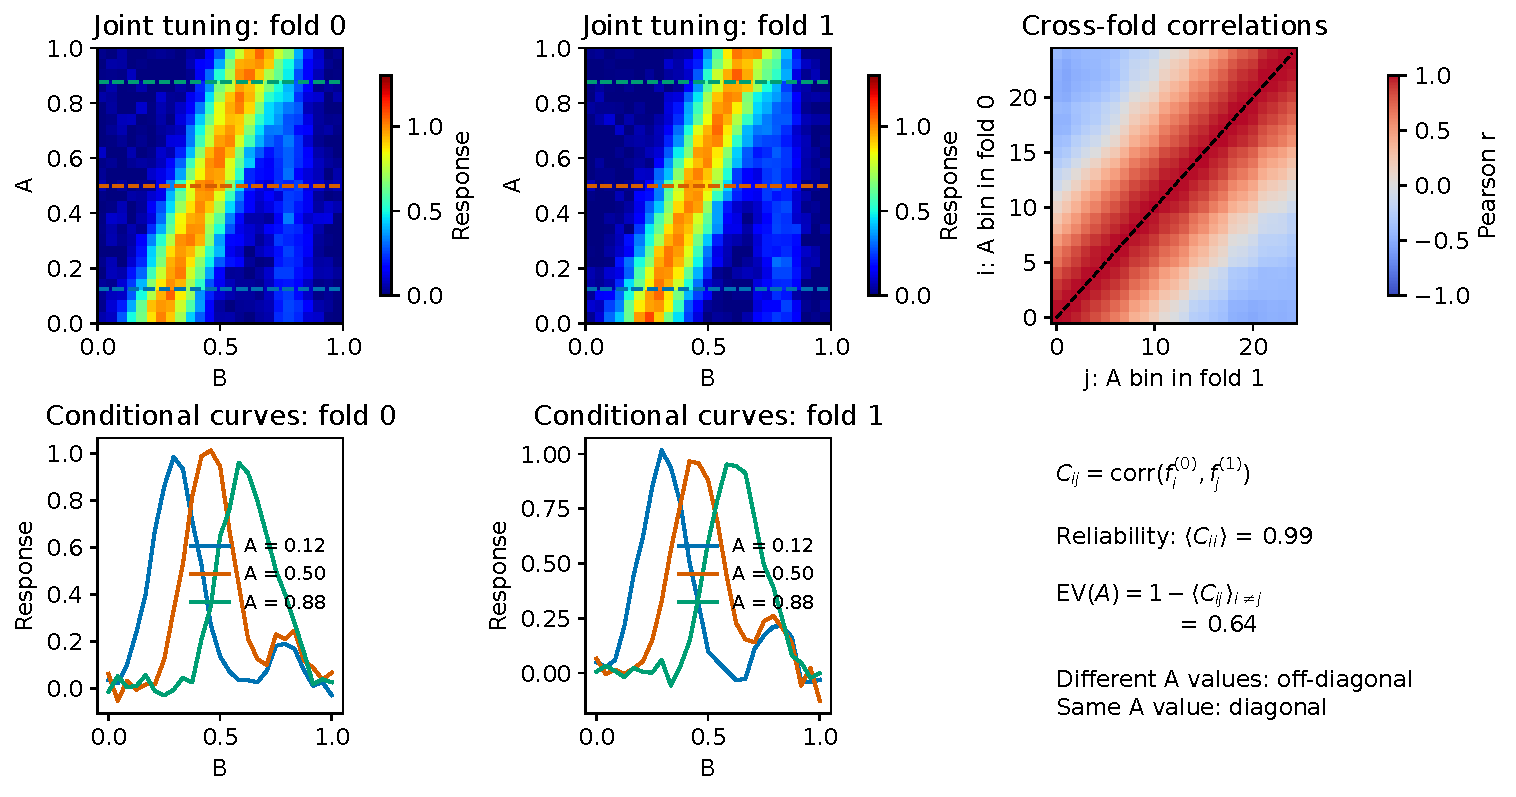
\includegraphics[width=.94\textwidth]{final_figures/method_schematic.pdf}\\[4pt]
    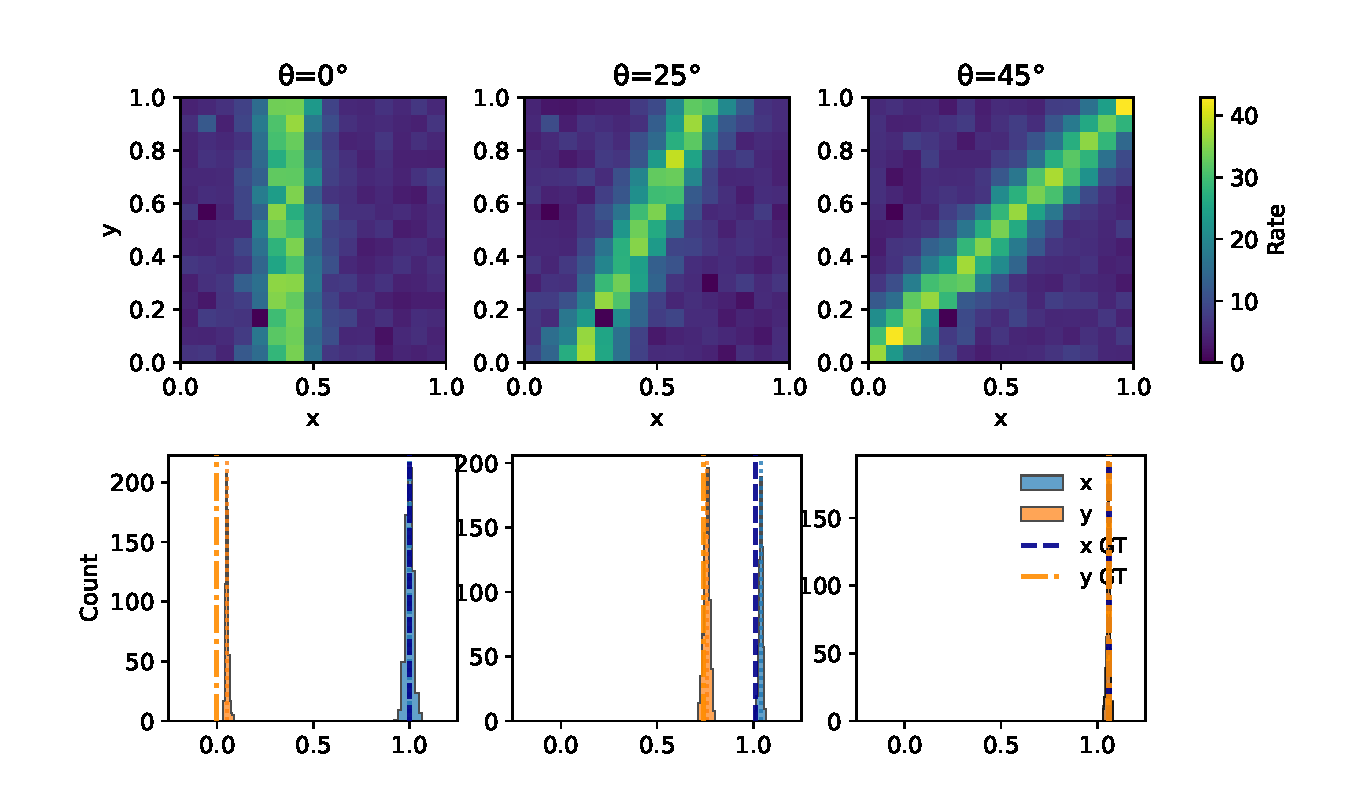
\includegraphics[width=.90\textwidth]{final_figures/estimator_validation.pdf}
    \caption{\textbf{Cross-fold correlations quantify conditional tuning shape.} All EV values are dimensionless, not percentages of explained variance. Top: joint maps from two folds are sliced at each value of $A$ to obtain tuning curves over $B$. Correlating fold-0 slice $i$ with fold-1 slice $j$ gives $C_{ij}$. Diagonal entries measure split-half reliability; $\mathrm{EV}(A)=1-\langle C_{ij}\rangle_{i\ne j}$ measures dissimilarity across different $A$ values. Bottom: simulated Poisson neurons with Gaussian-ridge log firing rates rotated by $0\degree$, $25\degree$, or $45\degree$, sampled on a $15\times15$ grid with 1,000 observations. Maps show one realization; histograms show EV for $x$ (blue) and $y$ (orange) across 600 datasets. Dashed lines mark noiseless reference values. EV can exceed 1 when conditional curves are anticorrelated. At $0\degree$, the invariant-axis estimate is close to the reliability-based noise reference; sampling sensitivity is shown in Supplementary Fig.~\ref{fig:si_floor}.}
\label{fig:estimation}
\end{figure}

We quantify the contribution of each variable from the joint tuning map, based on this intuition. To quantify the contribution of $x$, we ask how much the neuron's tuning over $y$ changes across values of $x$. We slice the joint tuning map at each value of $x$ to obtain tuning curves over $y$, and compute the Pearson correlation between tuning curves at different values of $x$. If these tuning curves are all similar, $x$ contributes little; if they differ, $x$ shapes the response. The contribution of $y$ is computed symmetrically by slicing along the other axis. Because Pearson correlation is invariant to positive scaling and offsets of each tuning curve, the measure captures changes in the shape of the tuning and is insensitive to pure gain or baseline modulation.

Tuning curves estimated from finite data are noisy, and noise lowers the correlation between tuning curves even when the underlying tuning is identical. To measure this effect, we estimate the joint tuning map separately from two halves of the data and correlate each tuning curve in one fold with each tuning curve in the other fold (Fig.~\ref{fig:estimation}, top). Correlations between tuning curves at different values of $x$ quantify how much the tuning changes with $x$. Correlations between tuning curves at the same value of $x$ quantify the reliability of the estimate: one minus this reliability provides a noise reference for an invariant neuron under comparable slice reliability and support (see Methods). This reference is not a universal lower bound.
In simulations with known ground truth, the estimates approach the noiseless reference values under the tested sampling conditions, and the invariant-axis estimate is close to the reliability-based noise reference at adequate sampling (Fig.~\ref{fig:estimation}, bottom; Supplementary Fig.~\ref{fig:si_floor}).

\subsection{Model units in deep network models based on vision exhibit entangled spatial tuning}

While many studies suggest that path integration is important for the formation of cognitive maps in the brain~\cite{Mcnaughton2006,Burak2009,Cueva2018}, recent studies reported place-cell-like responses in deep neural networks trained or pretrained to perform vision tasks alone~\cite{Luo2024,Gornet2024automated}. Gornet and Thomson~\cite{Gornet2024automated} reported that training a virtual navigation agent to predict the next image frame led to the formation of cognitive maps, with units in certain hidden layers selective to the agent's location, similar to place cells. Luo et al.~\cite{Luo2024} analyzed the responses of units in ResNet (pretrained on image classification, or untrained) in a spatial environment and reported that a large fraction of units throughout the network exhibit spatial selectivity to location or head direction. These studies~\cite{Luo2024,Gornet2024automated} examined the marginal tuning to these spatial variables separately, without examining their joint tuning.
We examine the joint tuning of units in the types of deep network models studied in~\cite{Luo2024,Gornet2024automated}, and then compare them with neurons in the rodent spatial navigation system.

{\bf Model units in networks trained on predictive coding exhibit entangled spatial tuning}
Inspired by prior work on predictive coding~\cite{Srinivasan1982predictive,Rao1999predictive}, Gornet and Thomson~\cite{Gornet2024automated} trained a virtual navigation agent, implemented as a deep neural network, to predict the next image frame in a sequence of images as the agent moves in space and found place-cell-like responses in its intermediate layers.

We trained this model on smooth, heading-aligned trajectories in Minecraft, following the released SGD/OneCycle recipe while correcting normalization to operate independently on each frame (Methods). On held-out trajectories, next-frame mean-squared error was $70.0\%$ below copying the current frame; providing the real history reduced error by $53.3\%$ relative to repeating the current frame. We examined units in four layers of this trained model. Because the head direction of the agent varies, we obtain the response of each unit for every combination of 2-D location and head direction.
Using established place-field criteria~\cite{Tanni2022}, a fraction of units in the intermediate layers are classified as putative place cells (Fig.~\ref{fig:pred}), consistent with~\cite{Gornet2024automated}. The joint tuning to location and head direction of these units is complex and entangled (Fig.~\ref{fig:pred}). When conditioned on different head directions, the location tuning maps change (Fig.~\ref{fig:pred}): the location selectivity of these units is not invariant to head direction.

Quantifying the contributions of location and head direction with the method above, location and head direction contribute about equally to the responses of most units (Fig.~\ref{fig:pred}; pre-prediction layer: median $\mathrm{EV}_{xy}=0.93$, median $\mathrm{EV}_{hd}=0.91$; $7{,}778$ of $8{,}000$ sampled units have finite scores on both axes, and $53.3\%$ of those have $\mathrm{EV}_{xy}>\mathrm{EV}_{hd}$). Units classified as putative place cells (red) fall in the same region as the other units.
The same holds in the other layers we analyzed, from the first convolutional layer to the output of the attention blocks (Supplementary Fig.~\ref{fig:si_pred_ev}).

\begin{figure}[p]
\centering
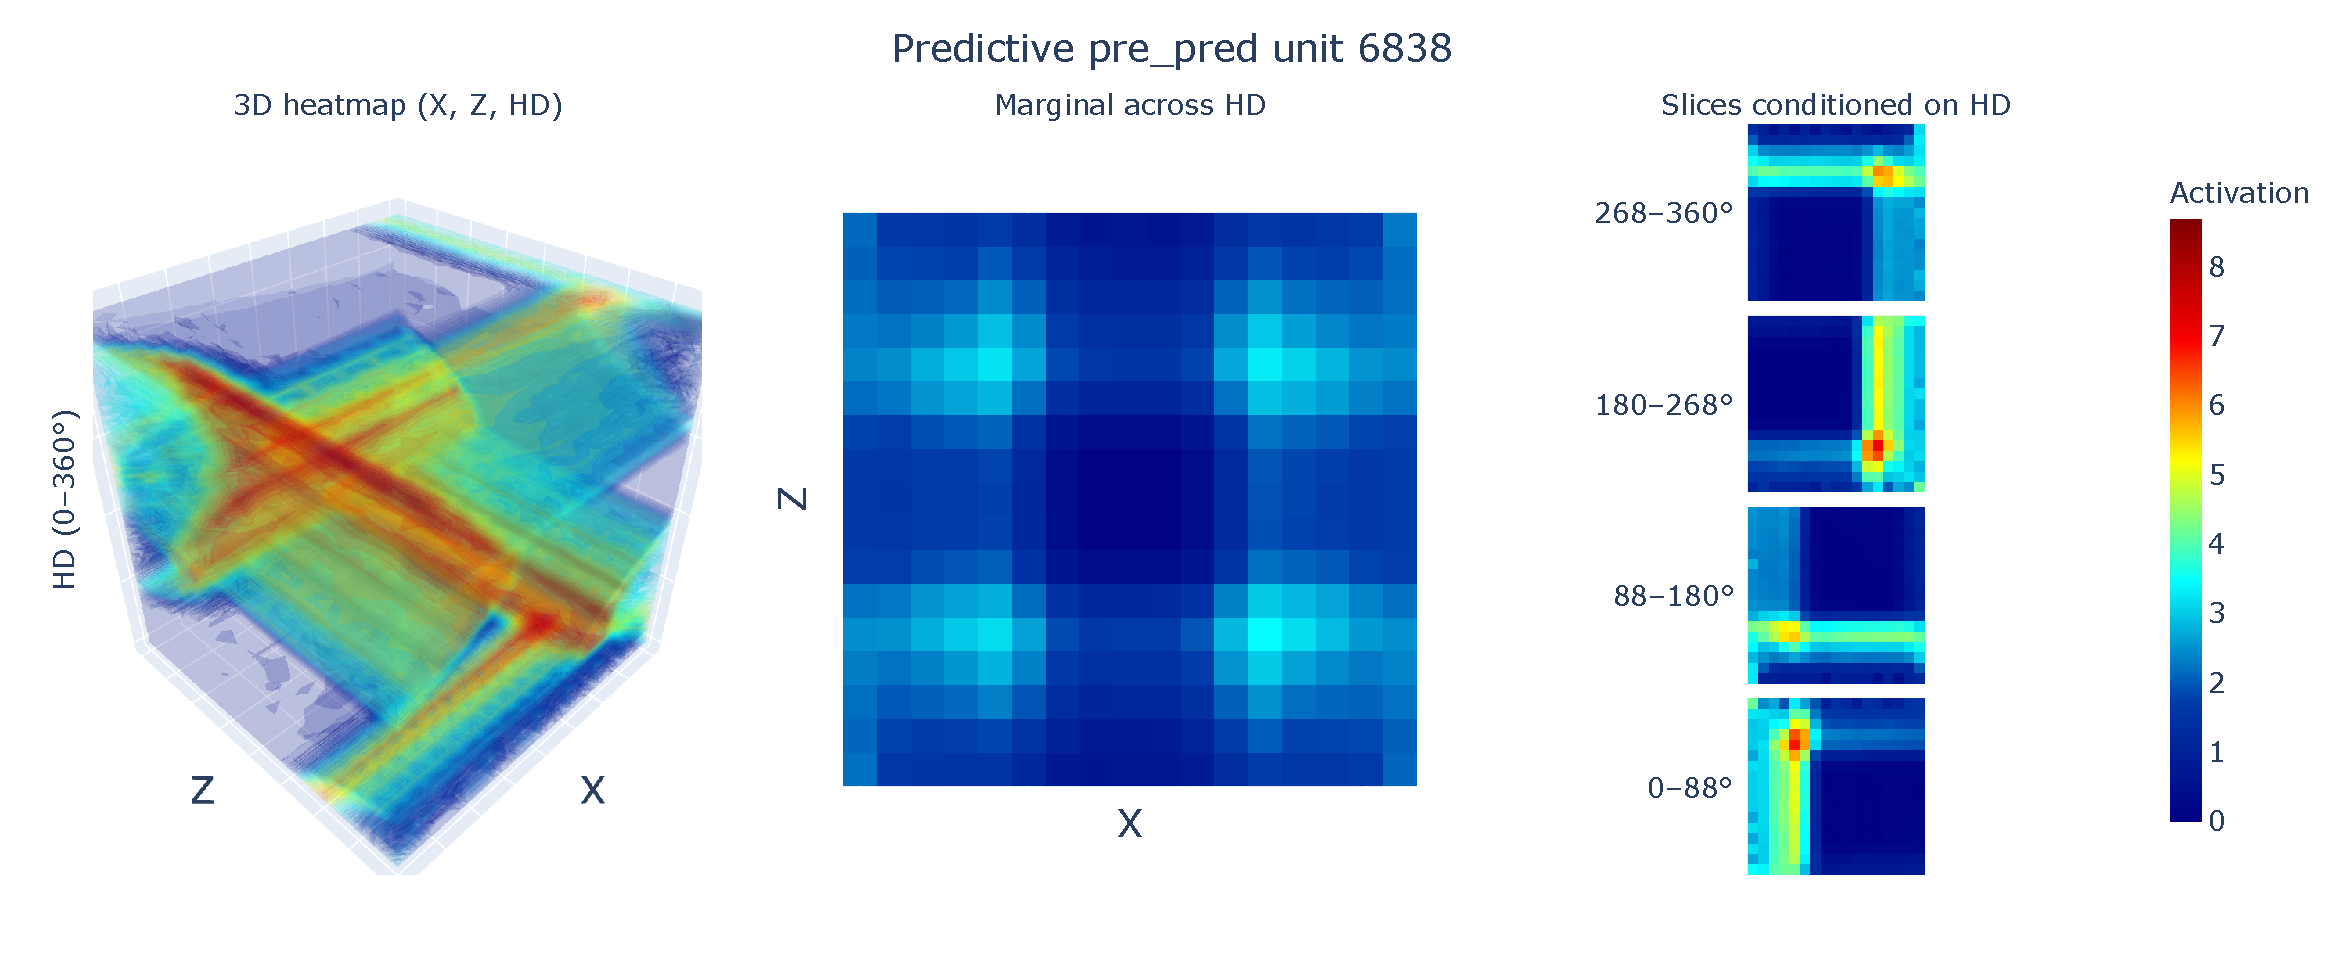
\includegraphics[width=.90\textwidth]{final_figures/pred_pre_pred_example.pdf}\\
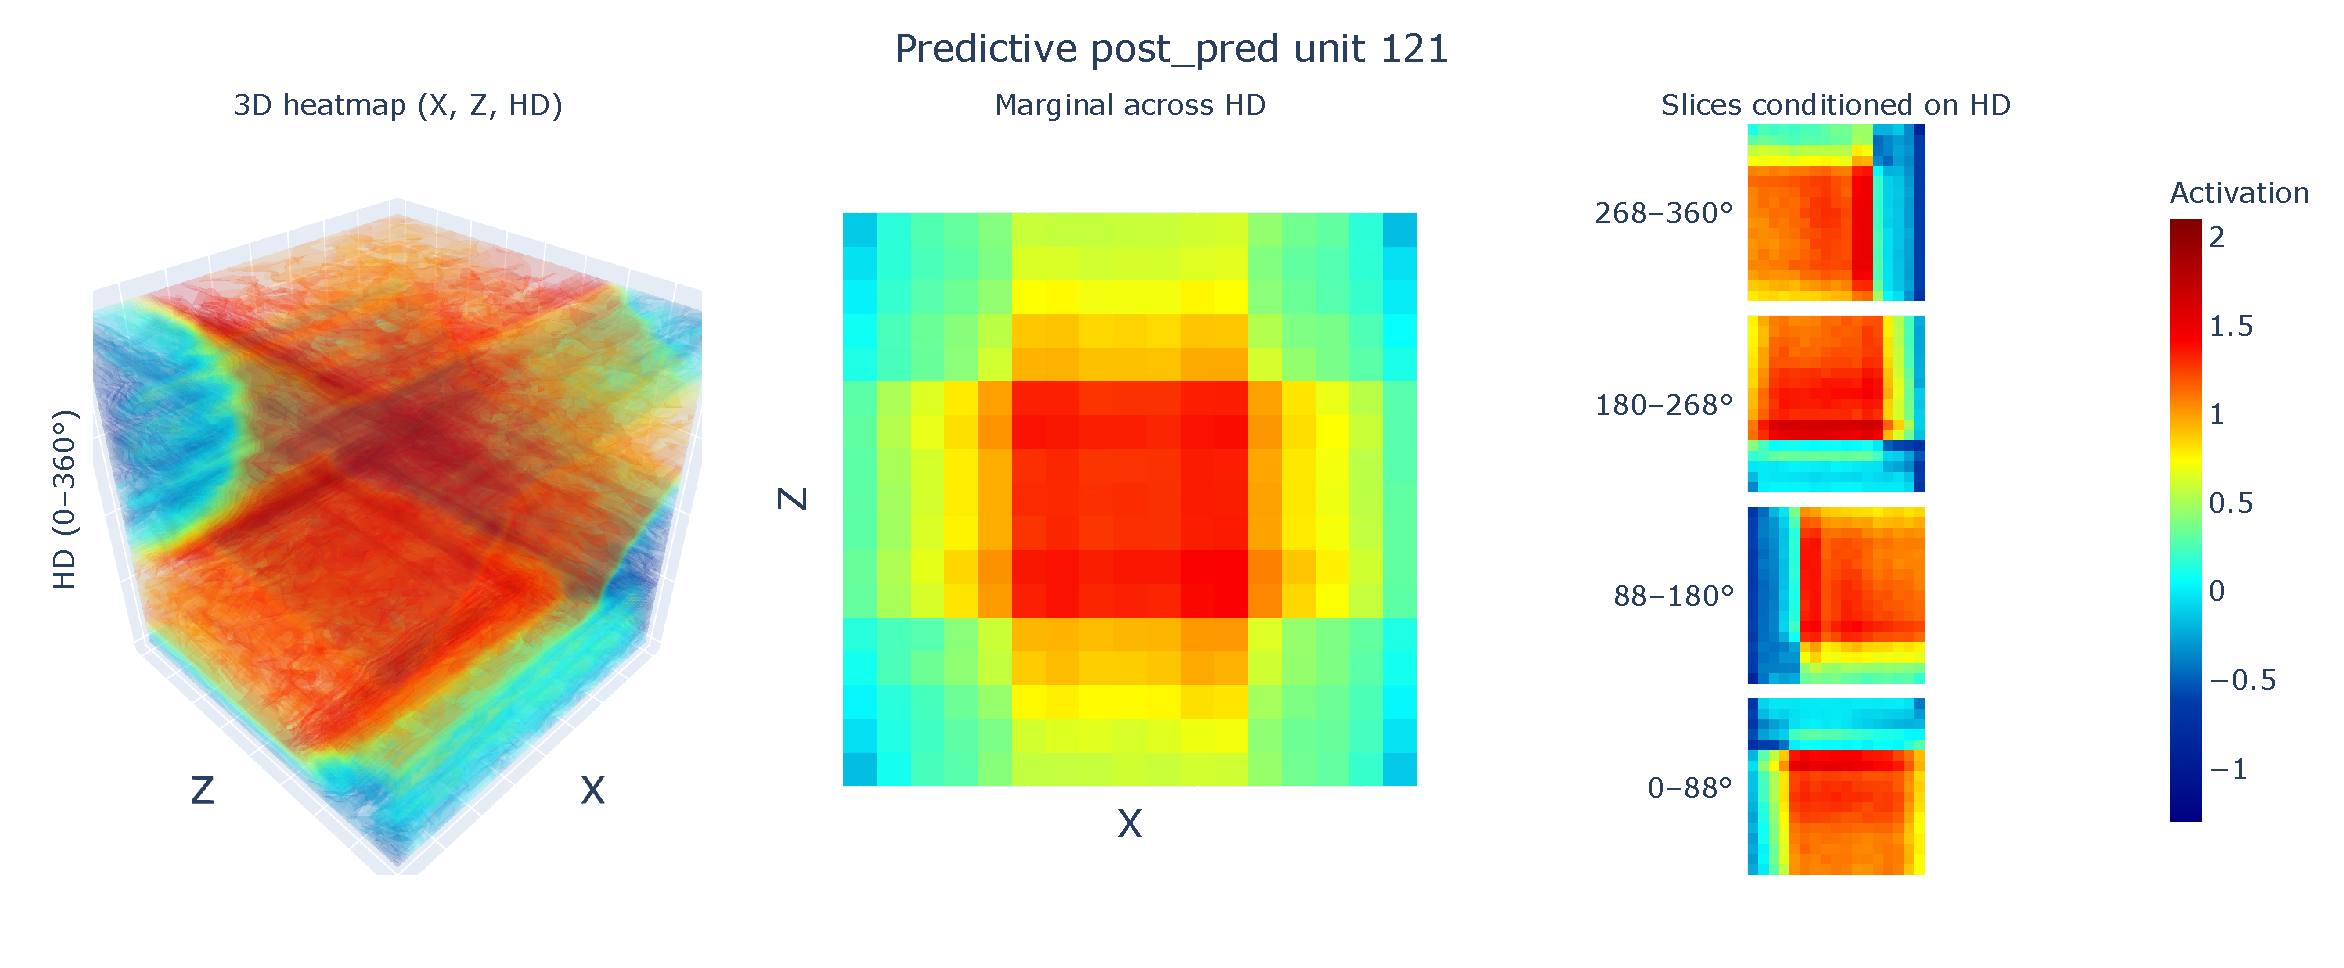
\includegraphics[width=.90\textwidth]{final_figures/pred_post_pred_example.pdf}\\
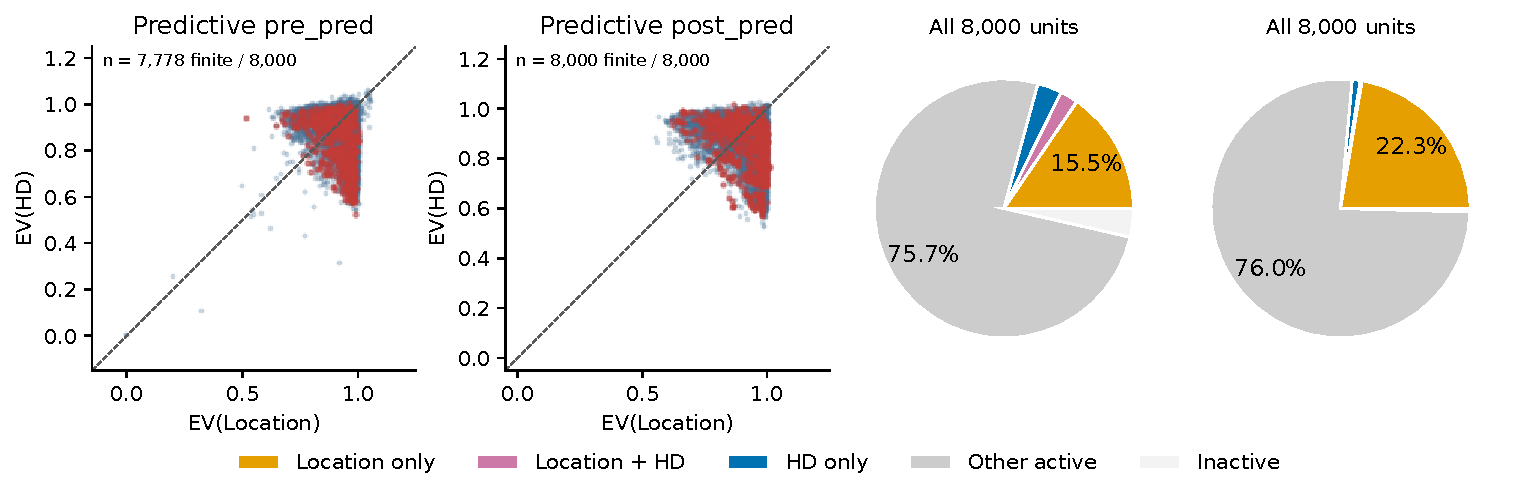
\includegraphics[width=.96\textwidth]{final_figures/pred_summary.pdf}
\caption{\textbf{Predictive-coding units exhibit entangled location and head-direction tuning.} Top rows: an exclusive place-classified unit from each latent layer, chosen randomly within that category. Each row shows the joint location$\times$HD map, the mean over HD, and four HD-sector maps, with shared activation limits. Bottom: EV scatter plots (left pair) and classification pies (right pair) for the pre- and post-prediction layers. Location-selective categories combine place and border criteria; the location-plus-HD category also meets the HD criterion. Red scatter points retain the exclusive place subset. Pies include all sampled units; scatter plots omit undefined correlations and report finite denominators. Axis limits include all finite points. Full category and layer breakdowns are in the supplement.}
\label{fig:pred}
\end{figure}

{\bf Pretrained convolutional neural networks (CNNs) also exhibit entangled spatial tuning}  We next investigate deep neural networks pretrained to perform image classification. Convolutional neural networks (CNNs) are a popular modeling framework for how the brain processes visual information~\cite{Yamins2014,Khaligh2014,Yamins2016}. Luo et al.~\cite{Luo2024} proposed using CNNs to study the navigation system in the brain. They modeled the visual inputs of a virtual agent navigating a 2-D open arena similar to the environments of rodent neurophysiology experiments. These CNNs are pretrained on visual tasks and receive only visual inputs, with no input about the agent's velocity. Luo et al.~\cite{Luo2024} reported that many units throughout the network exhibit place-cell-like responses as well as head direction tuning.

\begin{figure}[p]
\centering
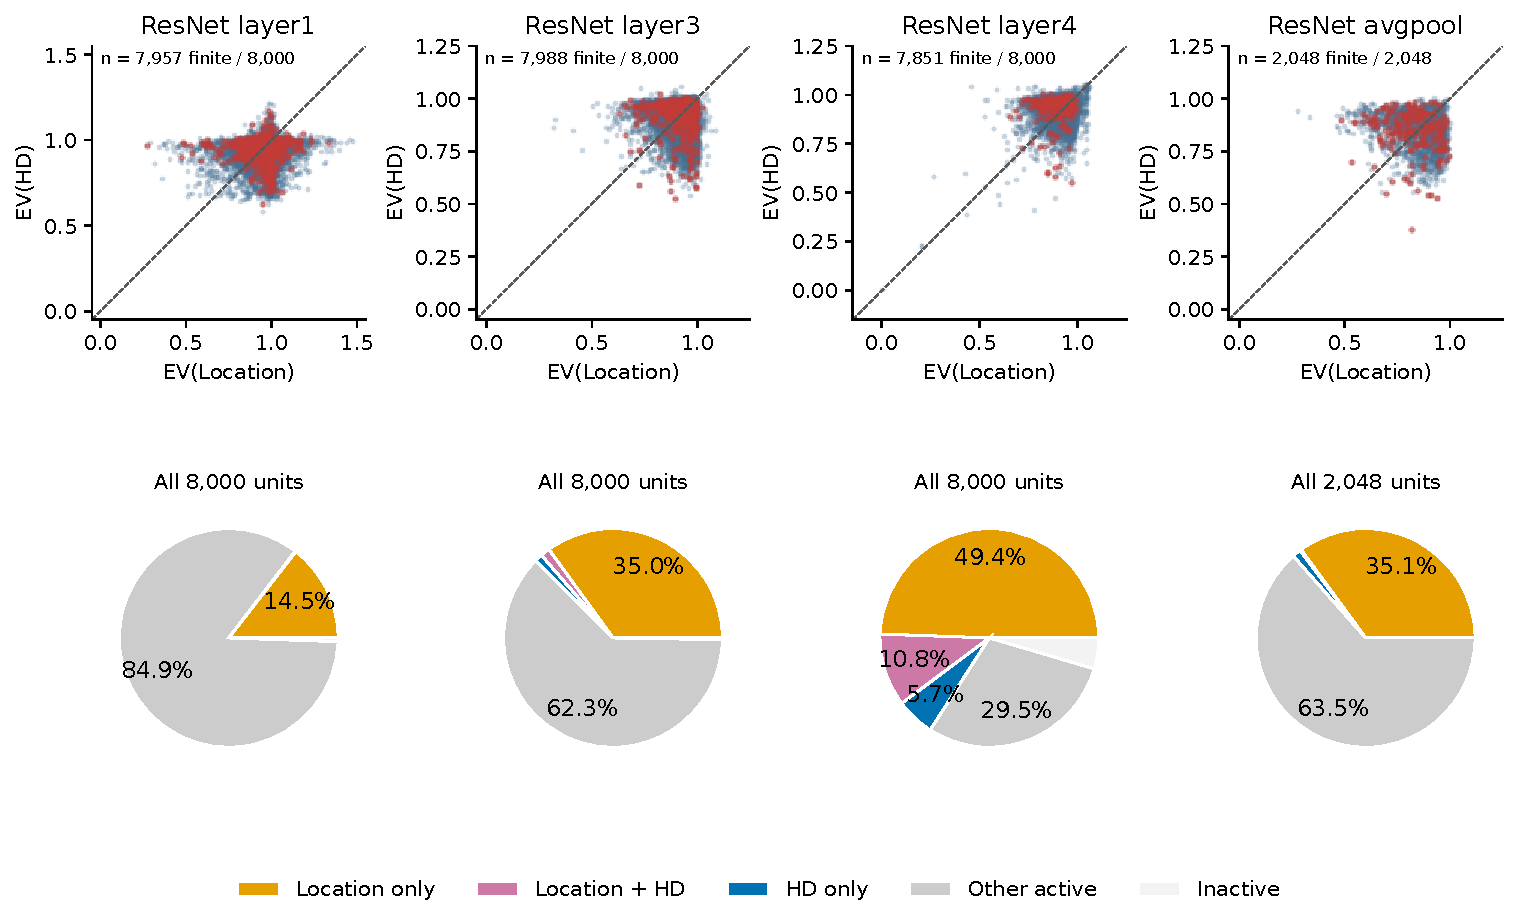
\includegraphics[width=.98\textwidth]{final_figures/cnn_main.pdf}
\caption{\textbf{ResNet-50 units show joint dependence on location and head direction.} Top: EV scatter plots in four ImageNet-pretrained layers; red points are exclusive place-classified units. Limits vary to include all finite scores. Bottom: disjoint classification groups combining place and border criteria into location selectivity. The same panorama images and pitch-fold definitions are used for the predictive model and CNNs. Supplementary figures retain the detailed categories, other architectures, and example joint maps.}
\label{fig:CNN}
\end{figure}

We analyzed a ResNet-50~\cite{He2016} pretrained on image classification in the same Minecraft environment used for the predictive coding network, which is similar to the environment of~\cite{Luo2024}. Consistent with~\cite{Luo2024}, a fraction of units exhibit putative place fields in 2-D space. Luo et al.~\cite{Luo2024} also reported that many units exhibit strong head direction tuning and that a subset exhibit conjunctive place and HD tuning. In our analysis of marginal tuning, few units are tuned to HD, and consequently few units are tuned to both HD and location. In the code released with~\cite{Luo2024}, the criterion for head direction cells does not properly capture selectivity to head direction: applying that criterion to our network also classifies many units as head direction cells. Applying the alternative criterion to the same responses changes the prevalence of HD classifications, demonstrating sensitivity to the classification rule. This within-data comparison does not isolate every difference between studies.

The joint location$\times$HD maps of units classified as putative place cells show firing fields scattered through the 3-D space (Supplementary Fig.~\ref{fig:si_scattered_maps}): a unit is active only for particular combinations of location and HD, as in the network trained on next-frame prediction. Across all layers, location and head direction contribute about equally to the responses of individual units (Fig.~\ref{fig:CNN} for four layers of ResNet-50; Supplementary Fig.~\ref{fig:si_cnn_ev} for VGG-16~\cite{Simonyan2015} and an untrained ResNet-50).

Together, these results reproduce key findings of recent studies of spatial tuning in deep neural networks trained on purely visual tasks: in the marginal tuning to 2-D location, a fraction of units have putative place fields. The joint tuning, however, shows that location and head direction are strongly entangled in these models. For most units, location and head direction contribute about equally to the response, rather than showing the opposing population preferences observed in the biological datasets.

\FloatBarrier
\subsection{Distinct selectivity and invariance of place cells and head direction cells in rodent brain}

We next analyze neurons recorded in the rodent spatial navigation system and compare them to the deep network models. We analyze two datasets: putative excitatory CA1 neurons recorded while rats navigated a 2-D open arena~\cite{Pfeiffer2013}, and head direction cells recorded from the postsubiculum of mice~\cite{Duszkiewicz2024}. Beyond the selectivity that defines each cell type, we ask whether these cells are invariant to the other spatial variables, e.g., whether place cells are invariant to head direction.

\textbf{CA1 tuning shapes depend more strongly on location than on head direction} We computed the 2-D firing rate maps of putative excitatory CA1 neurons from~\cite{Pfeiffer2013} ($n=551$ neurons from four rats). Consistent with previous reports, many of these neurons are selective to location in the open arena, with compact place fields, and most do not exhibit strong marginal tuning to head direction.
As shown above, marginal tuning alone does not establish invariance to another variable. We therefore computed the joint tuning map for location and HD, a 3-D map for each neuron (Fig.~\ref{fig:PlaceCell}). The example cells show localized spatial activity in their joint maps, with variation across head-direction sectors. Pure positive gain changes do not contribute to the correlation-based score; changes in spatial tuning shape do.

\begin{figure}[p]
\centering
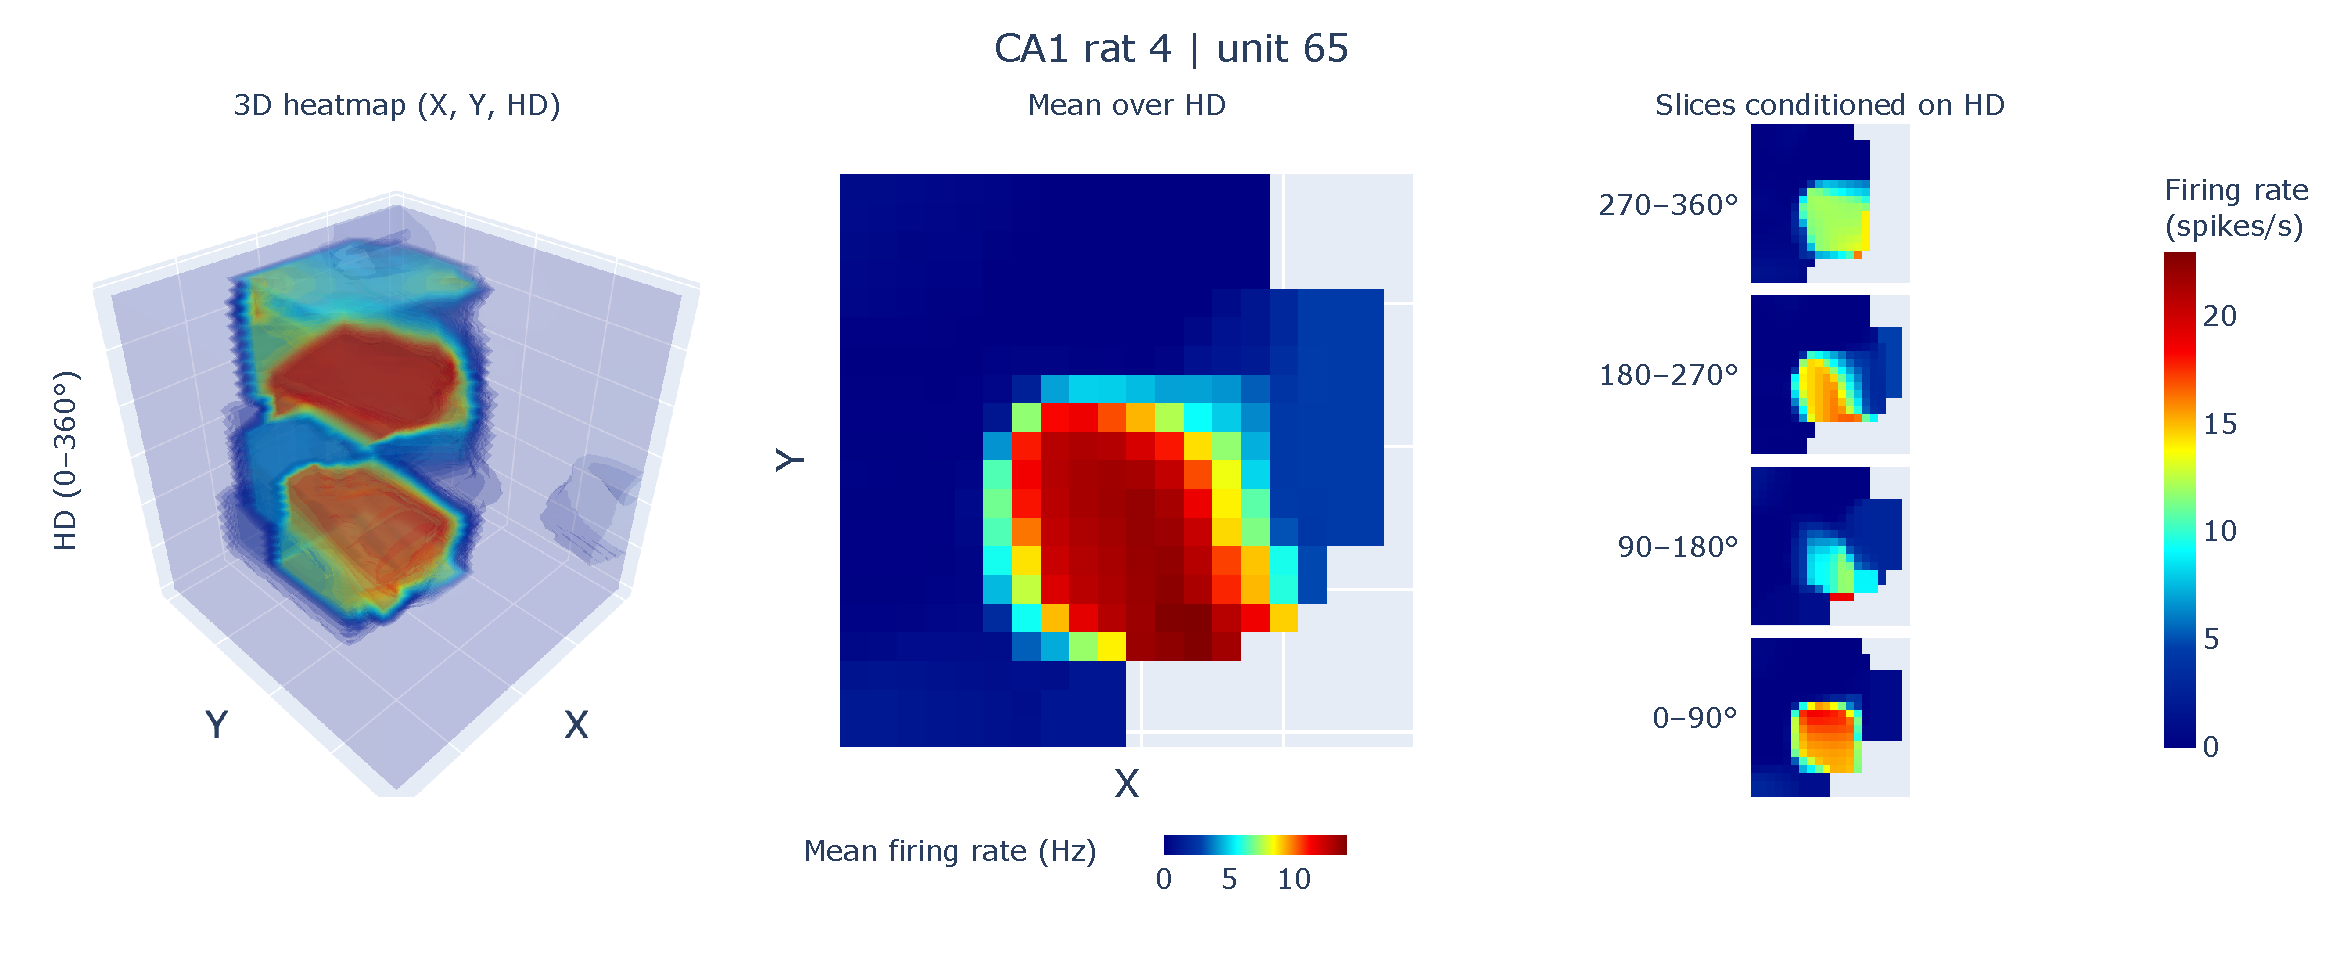
\includegraphics[width=.90\textwidth]{final_figures/pfeiffer_4_63.pdf}\\
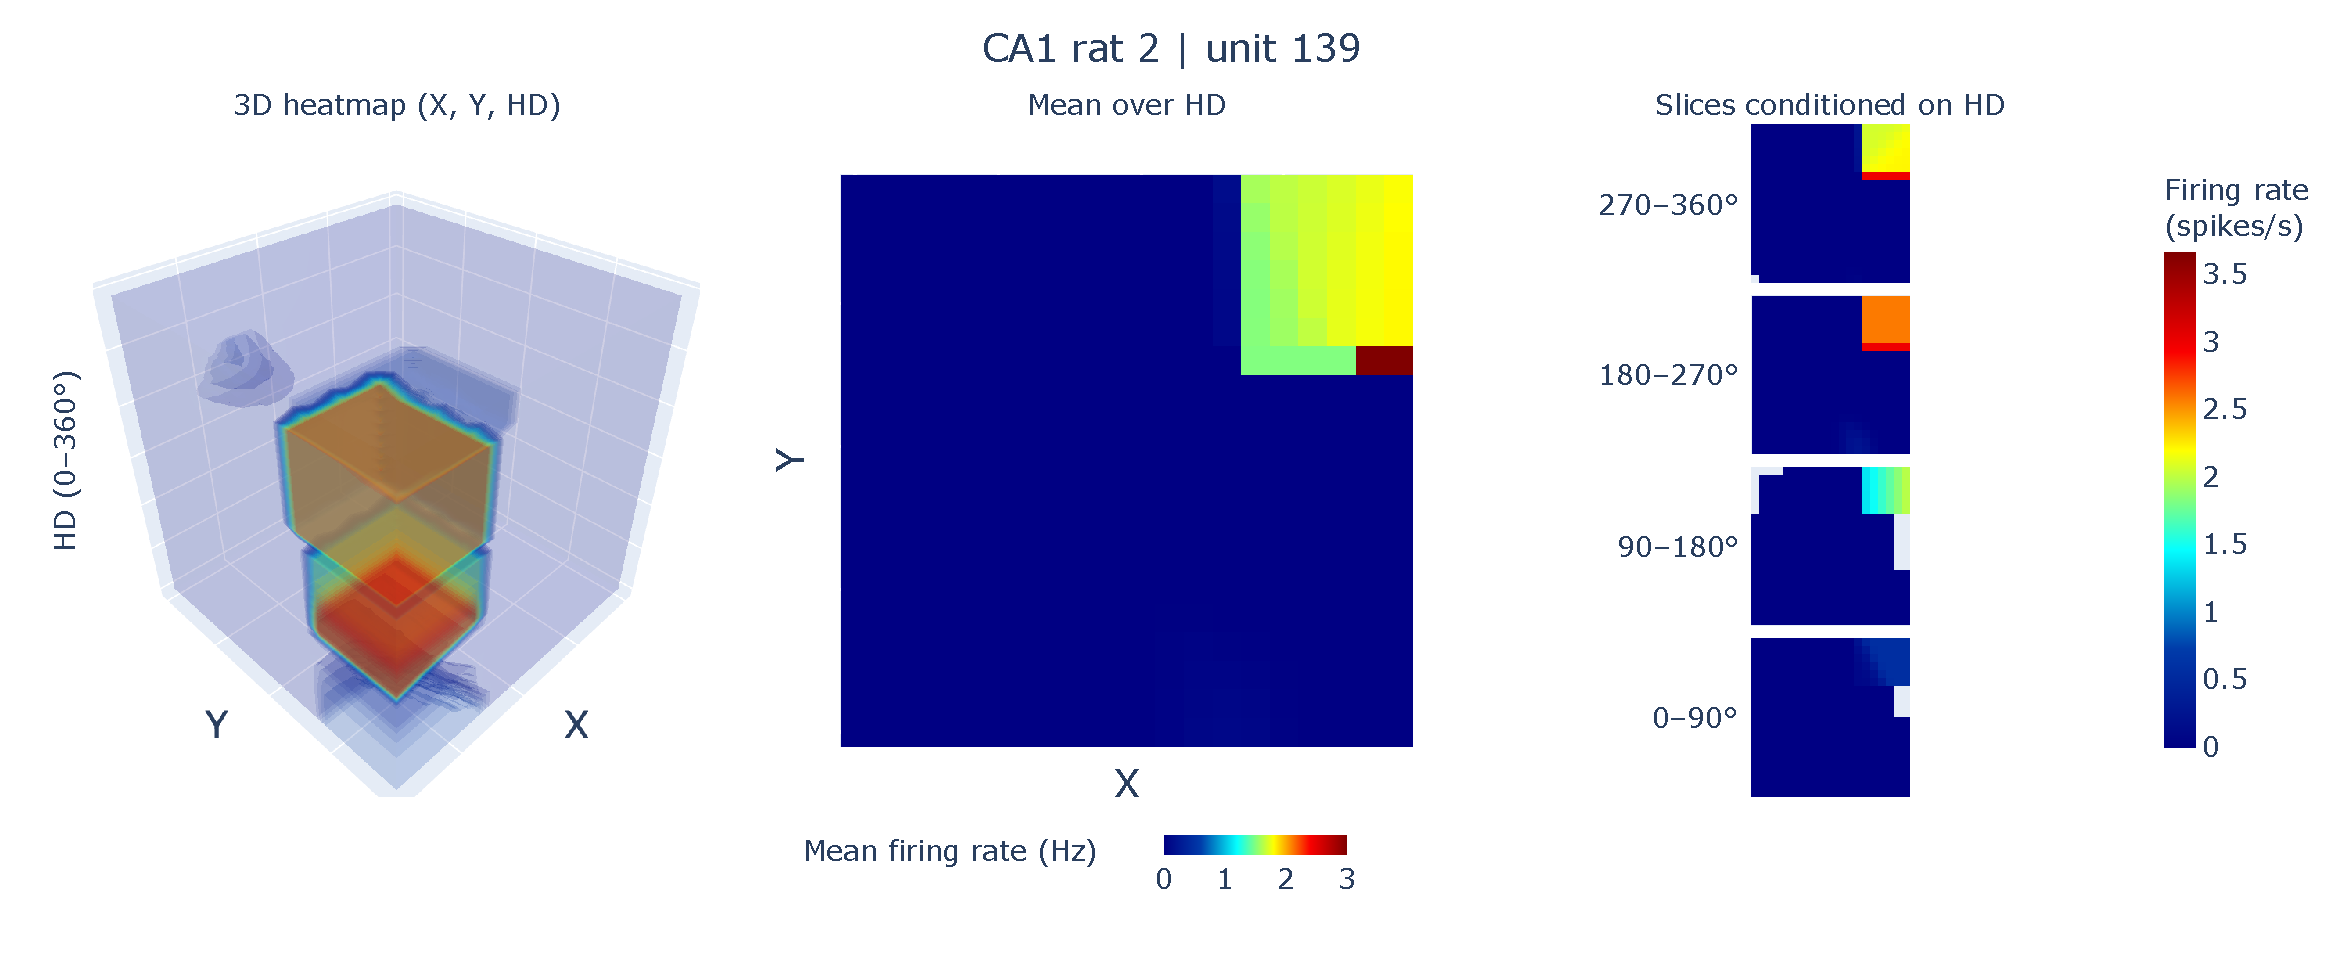
\includegraphics[width=.90\textwidth]{final_figures/pfeiffer_2_133.pdf}\\
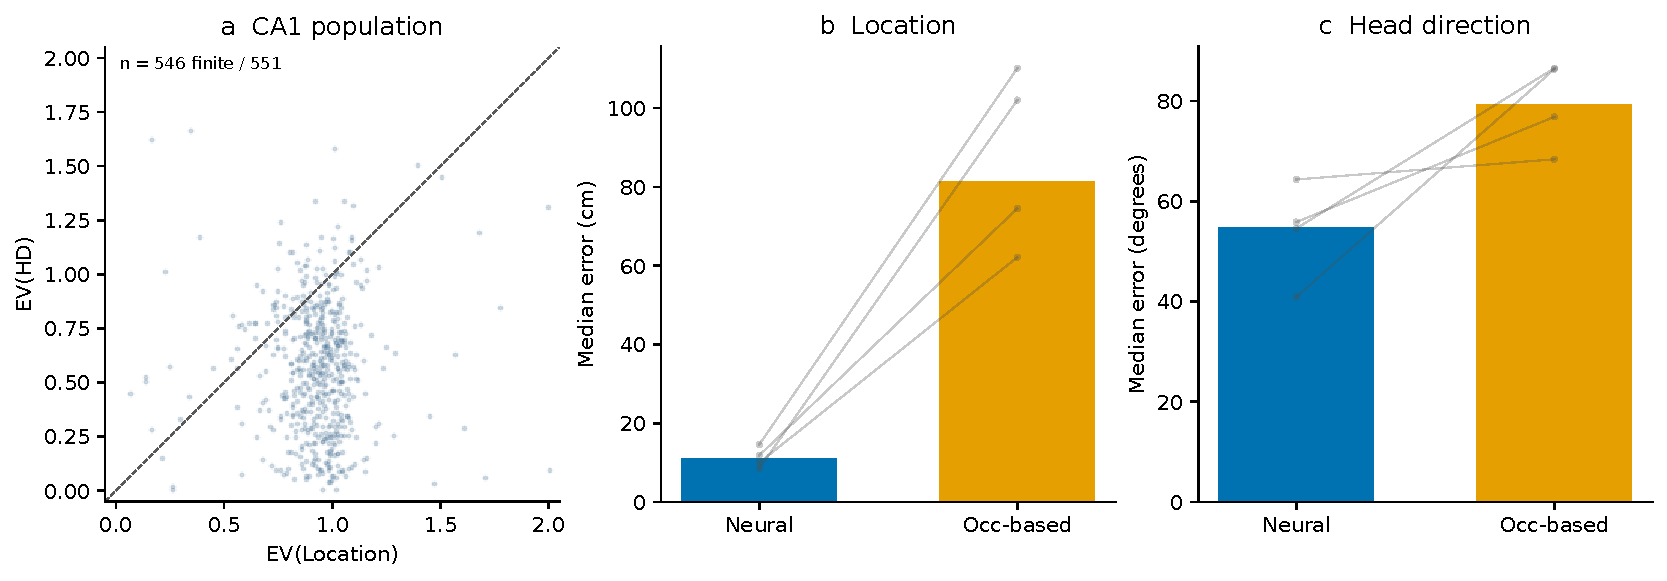
\includegraphics[width=.96\textwidth]{final_figures/ca1_summary.pdf}
\caption{\textbf{CA1 neurons show stronger tuning-shape dependence on location than on HD.} Top rows: identified example cells from rats 4 and 2, with joint maps, HD-averaged maps, and HD-sector maps. Coordinates are spatial-bin indices; the mean map uses its own zero-based Hz scale, while joint and sector maps share a scale. Bottom: (a) scores for all finite neurons, including values above 1; (b,c) held-out location and HD decoding. Bars are pooled medians over held-out bins; connected gray points are each rat's median errors. The occ-based baseline reports the most occupied training bin.}
\label{fig:PlaceCell}
\end{figure}

We quantified tuning-shape dependence on location and head direction (Fig.~\ref{fig:PlaceCell}). Location has the larger score in $85.2\%$ of the $546$ neurons with finite estimates on both axes ($551$ analyzed; median $\mathrm{EV}_{xy}=0.95$, $\mathrm{EV}_{hd}=0.57$). The median HD reliability reference is $0.47$. Reliability-normalized scores retain the preference (paired finite medians $0.76$ for location and $0.15$ for HD), although this normalization is not an unbiased decomposition of response variance.

The CA1 populations decode location with a pooled held-out median error of $11.2$~cm, compared with $81.3$~cm for the occupancy-based baseline. Head direction is also decoded better than that baseline ($54.7\degree$ versus $79.3\degree$; all four rats improve on both variables). Thus the weaker single-cell HD shape dependence does not imply an absence of population HD information.

\textbf{Postsubicular HD cells show the opposite preference} For the $1{,}489$ excitatory HD cells from 30 sessions of~\cite{Duszkiewicz2024}, the curated tracking release yields greater dependence on HD than location in $84.1\%$ of cells (median $\mathrm{EV}_{hd}=0.90$, $\mathrm{EV}_{xy}=0.73$; Fig.~\ref{fig:HD}). Reliability-normalized medians are $0.74$ for HD and $0.50$ for location. The contrast is graded: these cells retain measurable location-dependent changes in their HD tuning shapes.

Head direction is decoded with a pooled median error of $8.7\degree$, versus $81.3\degree$ for the occupancy-based baseline. Location is also decoded better than the occupancy baseline ($33.4$ versus $43.8$~cm; 28 of 30 sessions improve). The decoder excludes locations with no supported training-rate estimates. Population decoding can exploit response magnitude and behavioral correlations as well as changes in tuning shape; it therefore answers a different question from the single-cell correlation statistic.

Together, the two biological populations show opposing preferences in tuning-shape dependence, while neither population is completely invariant to the secondary variable. The contrast persists without interpolation of the location$\times$HD maps (Supplementary sensitivity analysis).

{\bf Comparison of the deep network models and the rodent hippocampus} The joint tuning to head direction and location reveals a large discrepancy between model units and spatial cells in the brain. Model units exhibit comparable tuning-shape dependence on head direction and location, whereas CA1 and HD-cell populations show opposing preferences. These models based on visual inputs alone therefore do not account for the key properties of the spatial cells found in the brain, and the joint tuning of multiple variables provides a more informative signature than marginal tuning for testing such models.

\begin{figure}[p]
\centering
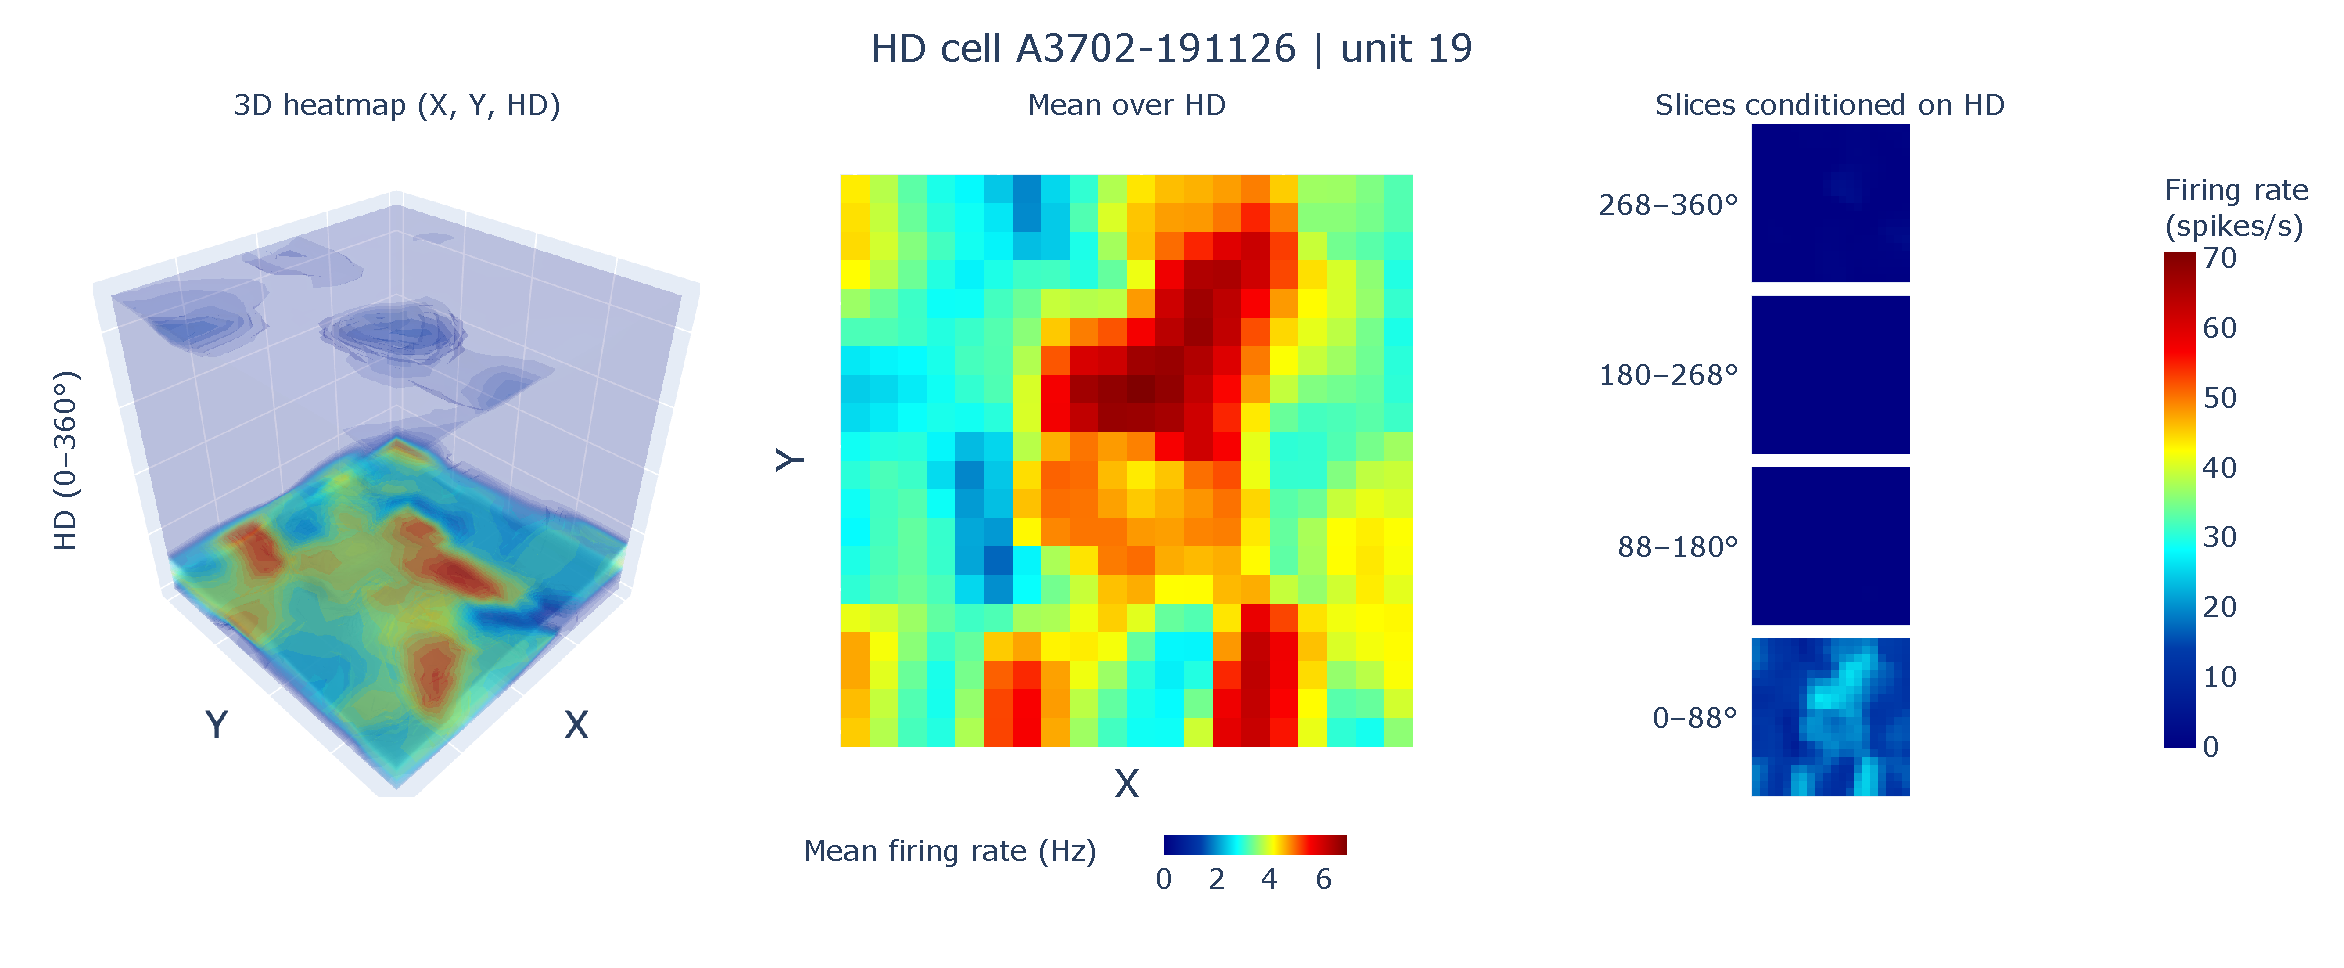
\includegraphics[width=.90\textwidth]{final_figures/dusz_A3702-191126_13.pdf}\\
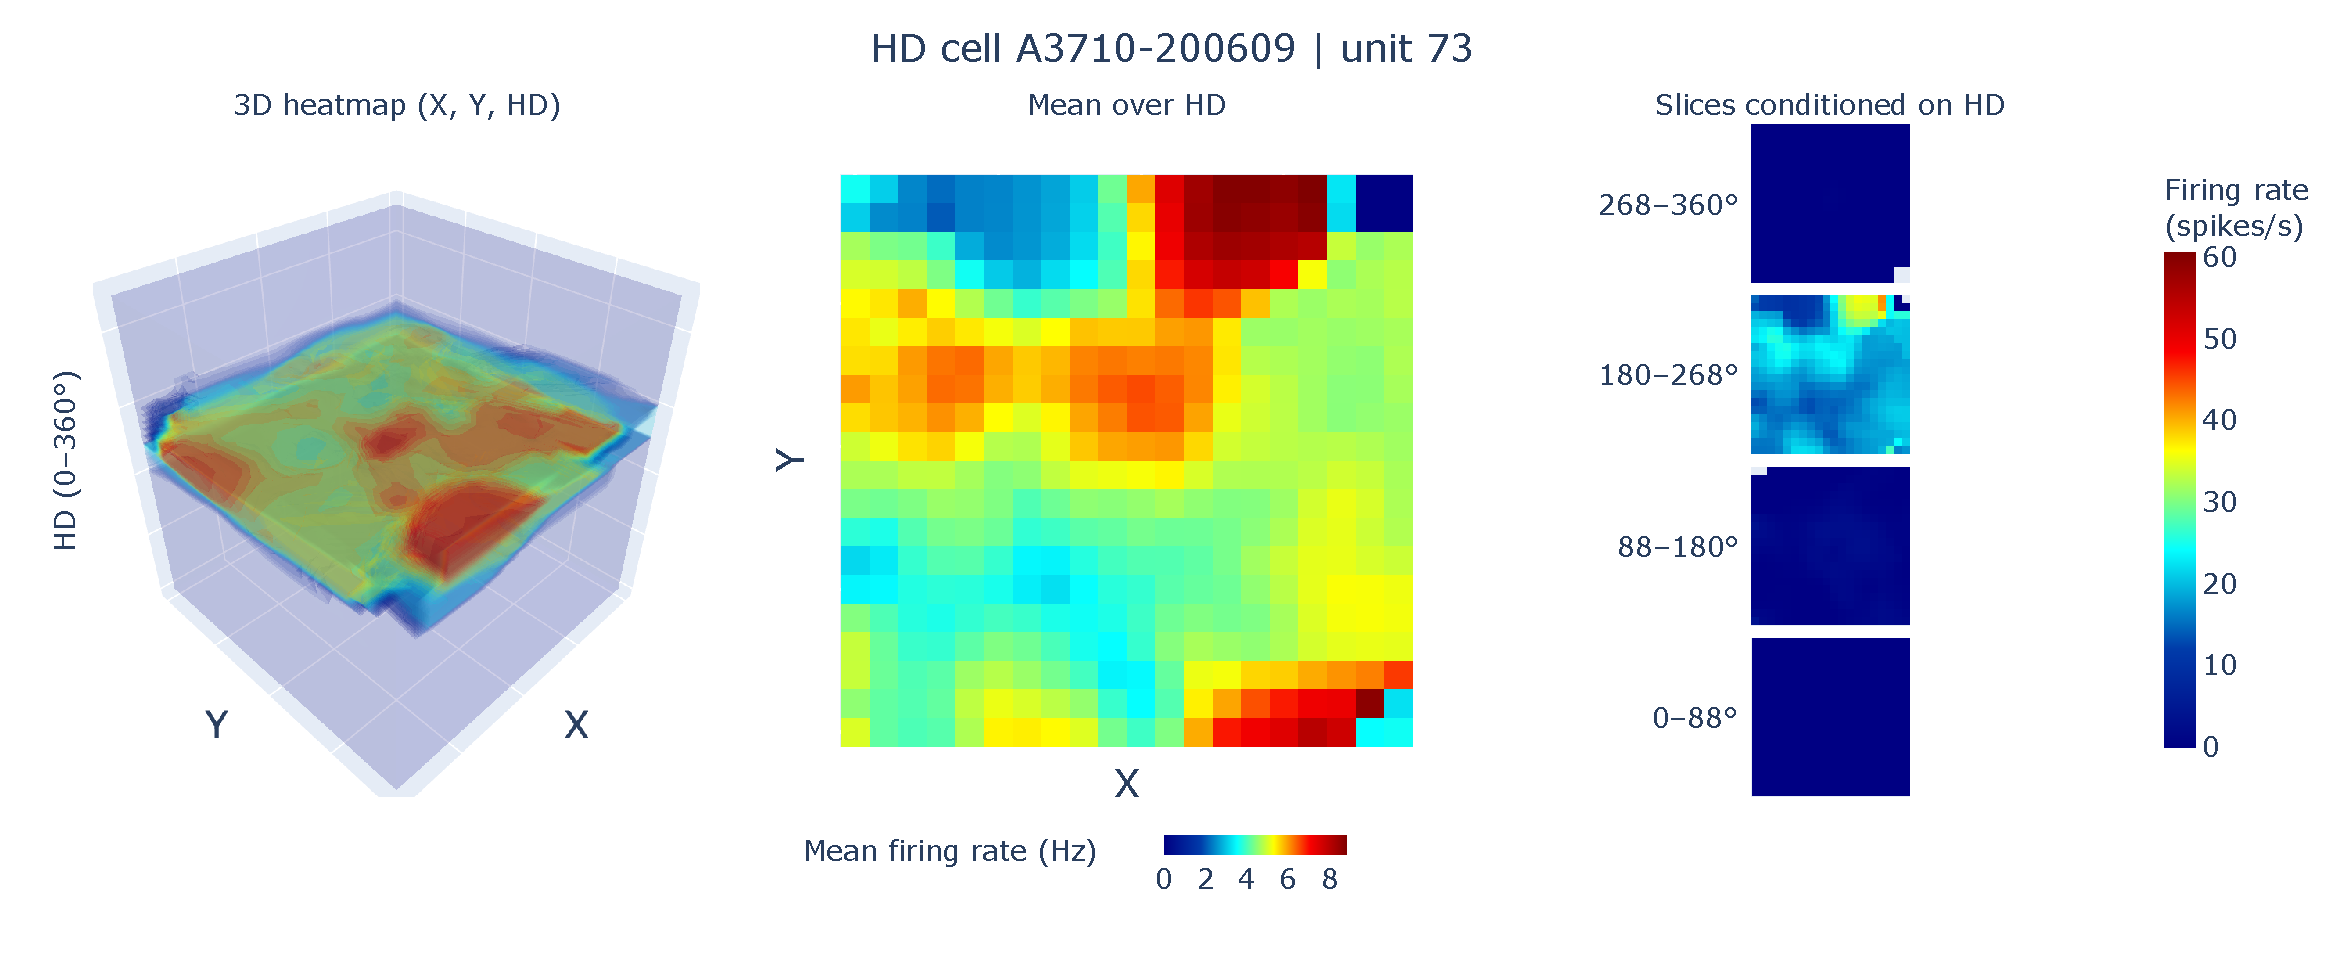
\includegraphics[width=.90\textwidth]{final_figures/dusz_A3710-200609_57.pdf}\\
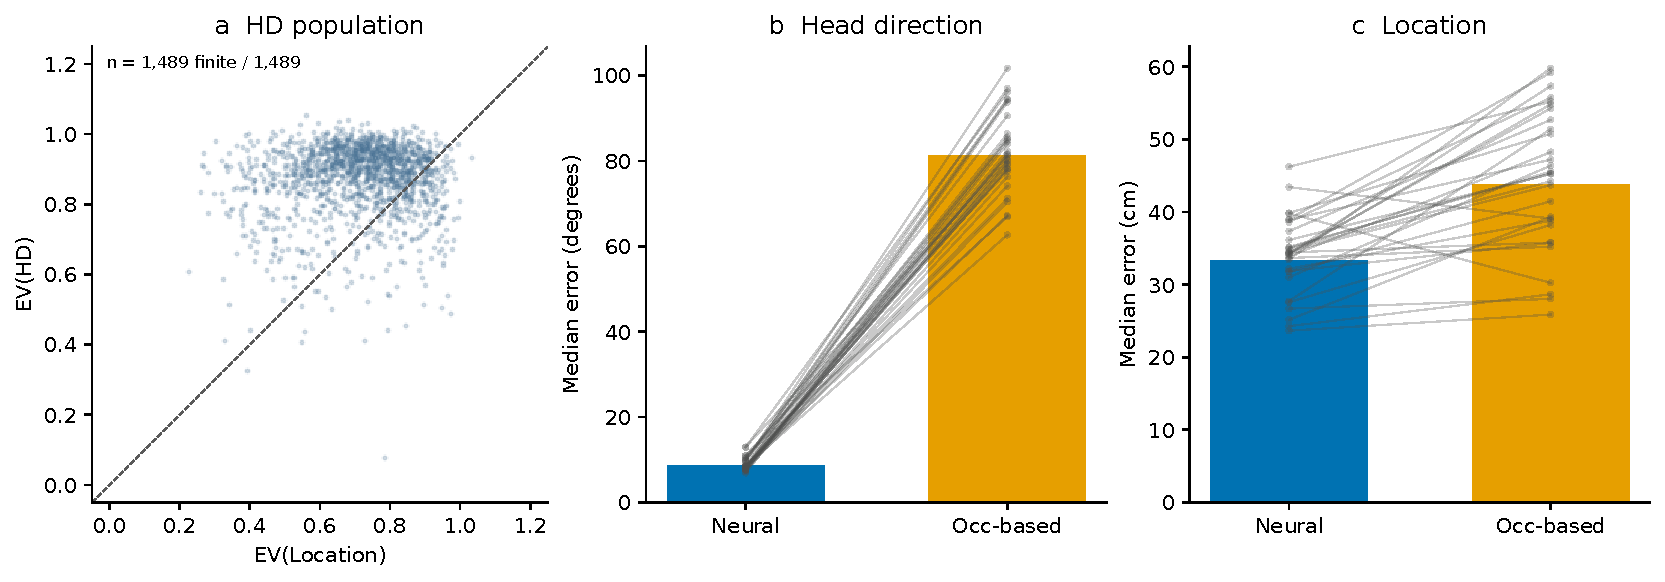
\includegraphics[width=.96\textwidth]{final_figures/hd_summary.pdf}
\caption{\textbf{HD cells show stronger tuning-shape dependence on HD than on location.} Top rows: identified cells from sessions A3702-191126 and A3710-200609, shown as in Fig.~\ref{fig:PlaceCell}. A low HD-averaged firing rate reflects averaging a narrow directional response over many directions; white regions lack supported estimates. Bottom: (a) scores for all $1{,}489$ cells; (b,c) HD and location decoding. Bars are pooled held-out medians and gray lines connect session medians. Both variables are decoded better than the occupancy baseline, despite their different single-cell shape dependence. The mean map uses its own zero-based firing-rate scale to reveal spatial spread; the joint and sector maps share a separate scale.}
\label{fig:HD}
\end{figure}

\subsection{Head direction dominates movement direction in postsubicular tuning and decoding}

The analysis of joint tuning applies beyond the comparison of deep network models and the hippocampus. We next use it to study a question that is central to understanding grid cells~\cite{Hafting2005,Stensola2012}. A popular class of computational models proposes that the hexagonal grid firing pattern results from path integration~\cite{Burak2009,Mcnaughton2006,Couey2013,Cueva2018}. This class of models requires that grid cells receive input about the animal's velocity (i.e., movement direction and speed). Neurons that encode movement speed have been identified in the entorhinal cortex and other areas~\cite{Kropff2015speed,Hinman2016}, but neurons that selectively encode movement direction have not been identified, and head direction is often assumed to stand in for movement direction.
Although the two are correlated, a previous study~\cite{Raudies2015head} found that (i) head direction is more strongly encoded in head direction cells than movement direction, and (ii) head direction and movement direction are sufficiently distinct that head direction would be an insufficient input for generating grid patterns in path integration models. It has remained unclear whether head direction cells are tuned to movement direction (MD) once the correlation between head and movement directions is taken into account, and whether the head direction population encodes a movement direction signal accurate enough for path integration.

We re-analyzed the head direction cells of~\cite{Duszkiewicz2024} to address these questions. A substantial fraction of these cells show marginal tuning to MD, which could reflect either selectivity to MD or the correlation between MD and HD.
To separate the two, we examined joint HD$\times$MD tuning using $10\degree$ bins, which retain finite estimates for all $1{,}489$ cells. HD and MD lie within $30\degree$ of one another in $30.65\%$ of eligible time bins, compared with $16.70\%$ under independence of the empirical angular marginals (Fig.~\ref{fig:MD}). The score for HD exceeds that for MD in every cell (median $\mathrm{EV}_{hd}=1.00$, $\mathrm{EV}_{md}=0.21$). The median MD reliability reference is $0.17$, and the paired reliability-normalized medians are $0.95$ for HD and $0.03$ for MD. Finer $4\degree$ binning retains the population preference but yields fewer finite estimates and higher MD scores, emphasizing the importance of sampling coverage.

MD decoding is substantially less accurate than HD decoding: its pooled median error is $61.4\degree$, compared with $89.8\degree$ for the occupancy baseline. These results establish a strong preference for HD over MD in this population. They do not establish whether a downstream circuit could combine this signal with other inputs to support path integration.

\begin{figure}[htbp]
\centering
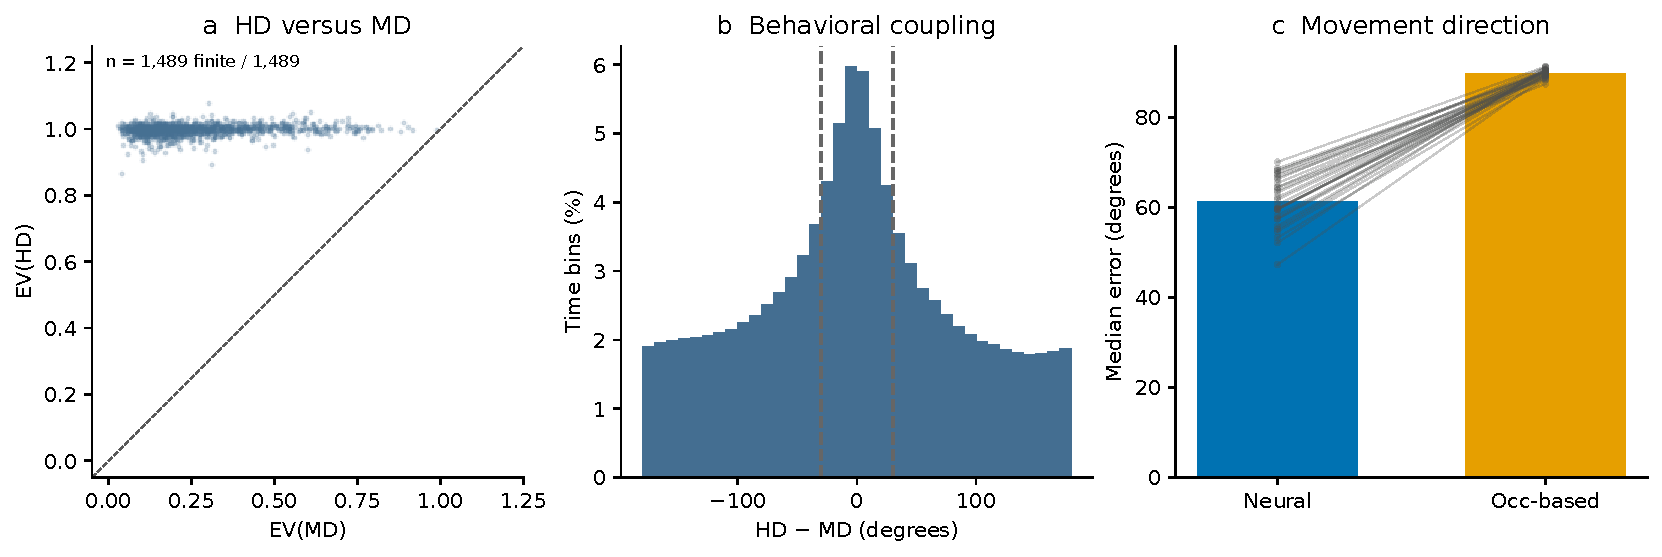
\includegraphics[width=.96\textwidth]{final_figures/md_summary.pdf}
\caption{\textbf{HD tuning and decoding dominate MD in the postsubicular population.} (a) Cross-fold scores from $36\times36$ joint HD$\times$MD bins at zero tracking lag. (b) Distribution of HD minus MD across eligible time bins; dashed lines mark $\pm30\degree$. (c) MD decoding: pooled held-out medians (bars) and paired session medians (gray lines), compared with the occupancy-based baseline.}
\label{fig:MD}
\end{figure}


\FloatBarrier
\section{Discussion}

Joint tuning to multiple stimulus variables contains information that the standard analysis of marginal tuning curves misses, and the selectivity and invariance of a neural code need to be studied together.
The joint tuning of neurons is often studied with GLMs~\cite{Pillow2008spatio,Hardcastle2017multiplexed}, which can compare models containing different predictors. With an exponential link, separate additive functions imply multiplicatively separable tuning; explicit interactions relax that restriction.
When many behavioral variables must be considered simultaneously, a GLM is an effective approach, since more flexible models cannot be fit with the available data. When only a handful of variables are relevant, our approach provides an alternative that makes no assumption about how the variables interact and can reveal structure in the code that a GLM with separate terms cannot. Our measure targets changes in the shape of the tuning across values of a variable; gain modulation is invisible to it and must be assessed separately.

The biological populations show opposing tuning-shape preferences: location dominates in CA1, and HD dominates in postsubiculum. Their secondary-variable dependence is smaller but nonzero. Preserved tuning shapes can support generalization across a nuisance variable even when gains change, although this study does not directly test a fixed downstream readout. The distinction between shape and response magnitude is essential to interpreting invariance.

Applying our approach to deep network models based on vision tasks~\cite{Luo2024,Gornet2024automated}, the tuning properties of individual units differ drastically from those of place cells and head direction cells in the rodent brain.
Individual model units encode entangled representations of head direction and location. Most model units do not exhibit clear marginal tuning to head direction, yet their response is strongly modulated by head direction through its interaction with location. These results hold for both types of deep network models~\cite{Luo2024,Gornet2024automated}.
One interpretation is that these units are selective to visual features, and spatial selectivity emerges because the visual features in the environment depend on location and head direction jointly.
Even a unit in an early layer of the network that behaves as an edge detector can exhibit location and HD tuning. Such selectivity is substantially different from that of head direction cells and place cells: the network units are much less invariant to head direction and location than place cells and head direction cells in rodents.
These results reveal a major gap in current deep neural network models trained on vision tasks as accounts of the tuning properties of the rodent spatial navigation system. An open question is what additional ingredients would make model units selective to location and invariant to head direction, as in rodents.

Our approach applies to the joint tuning of individual neurons to a small number of behavioral variables (2 or 3) without assumptions about how the tuning to different variables interacts (such as the multiplicative interaction of a GLM with separate terms for each variable). Applied to head direction cells, it reveals much stronger dependence on HD than MD. Determining whether this population can contribute to path integration requires testing downstream readout and integration together with other inputs~\cite{Mcnaughton2006}.
The same technique can address the selectivity of place cells on linear tracks to location, time, and distance traveled. Hippocampal neurons on linear tracks have been proposed to encode location, time, distance traveled, or a combination of these~\cite{Eichenbaum2014time,Chen2024}, and these factors are hard to disentangle because they are highly correlated in experiments. Our approach estimates the contribution of each factor from the joint tuning.

Our results also bear on the study of mixed selectivity~\cite{Rigotti2013}, which has been reported in many brain areas and tasks. Methodologically, our approach quantifies mixed selectivity through the joint tuning and the contribution of each stimulus variable. Our analysis of the deep network models further shows that mixed selectivity can arise from analyzing the wrong set of stimulus variables. In the deep network models examined here, many units in the first layer are oriented filters that encode the orientation of edges.
Analyzed in terms of spatial variables, these units exhibit complex nonlinear mixed selectivity, because the mapping between the visual feature and the spatial variables (location and head direction) is highly nonlinear: an edge of a given orientation appears in the receptive field of the unit only for particular combinations of location and head direction. Mixed selectivity in neural systems has been proposed to carry functional advantages for coding~\cite{Rigotti2013,Fusi2016neurons}; the example above shows that it can also arise from misidentifying the encoded features, which calls for care in interpreting responses that appear mixed selective.

This paper focuses on the response properties of individual neurons. An important question is what the observed selectivity and invariance imply at the population level. The tuning properties of individual neurons constrain population-level properties because they define the projection of the neural manifold onto the individual neuronal axes~\cite{Kriegeskorte2021}, but this relationship has mainly been studied for a single stimulus variable. Understanding the relationship between the joint tuning to multiple variables and the structure of the neural manifold is an important direction for future research.

\newpage

\section{Methods}

\subsection{Analysis of marginal tuning curves under correlated stimulus sampling}
Here we show how correlated sampling of the stimuli produces spurious tuning in the standard analysis of tuning curves. Consider the tuning of a neuron to variables $x$ and $y$, with joint tuning $h(x,y)$.

Assume that the marginal sampling distribution over $x$ is uniform and that the joint tuning factorizes, $h(x,y)=f(x)g(y)$. The marginal tuning curve for $x$ estimated by the standard averaging procedure is
$$
\hat{f}(x) = \int p(y|x)h(x,y)dy = \int p(y|x)f(x) g(y)dy =f(x)\int p(y|x)g(y)dy .
$$
If $x$ and $y$ are independent, the procedure recovers $f(x)\int p(y)g(y)dy$, which is proportional to $f(x)$. Otherwise, through the $p(y|x)$ term, the estimated marginal tuning curve for $x$ depends on $g(y)$.

Consider the special case where the neuron is invariant to $x$, i.e., $h(x,y)=h(y)$ is a narrow Gaussian function, so that the true tuning curve for $x$ is constant. If only $y=x$ is sampled (perfectly correlated sampling of the two stimuli), the estimated tuning curve is
$$
\hat{f}(x) = \int p(y|x)h(y)dy = \int \delta(y-x)h(y)dy=h(x).
$$
Relying on the marginal tuning curves, we would incorrectly conclude that the neuron is strongly tuned to $x$.

\subsubsection*{Simulation parameters for the marginal confound and GLM demonstrations (Figs.~\ref{fig:fig1} and \ref{fig:glm})}

For the marginal confound demonstration (Fig.~\ref{fig:fig1}), $h(x,y)=\exp[-x^2/(2\sigma^2)]$ with $\sigma=0.7$, and $(X,Y)$ is bivariate standard normal with correlation $\rho\in\{0,0.6,0.95\}$. The plotted marginal is the analytic conditional expectation
\[
E[h(X,Y)\mid Y=y]=\frac{\sigma}{\sqrt{\sigma^2+1-\rho^2}}\exp\left[-\frac{\rho^2y^2}{2(\sigma^2+1-\rho^2)}\right].
\]
For the GLM demonstration, $\lambda(x,y)=5\exp[-(x\cos\theta-y\sin\theta)^2/(2\cdot1.2^2)]$ with $\theta=60\degree$ or $45\degree$. Each model is fit to 20,000 Poisson observations at independent standard-normal stimuli and evaluated on 20,000 new observations. The additive model contains an intercept, $x,y,x^2,y^2$; the interaction model additionally contains $xy$. Marginals integrate over the actual standard-normal distribution using Gaussian quadrature, checked against the analytic integral. Conditional slices fix $y=1$.

\subsection{Estimating the contribution of individual stimulus variables}
For every bin of the joint firing rate map of $(x, y)$, the samples that fall in the bin are randomly split into two equal halves, and each half is averaged to give the two fold maps $f^{(0)}(x,y)$ and $f^{(1)}(x,y)$. With $x$ and $y$ discretized into $m$ and $n$ bins, we write $f^{(0)}_{i,j} = f^{(0)}(x_i, y_j)$ and $f^{(1)}_{i,j} = f^{(1)}(x_i, y_j)$.

To quantify the contribution of $x$, we ask how much the tuning over $y$ changes across values of $x$. For each bin $x_i$, we take the tuning curve over $y$ at $x = x_i$, $\mathbf{f}^{(0)}_i = f^{(0)}(x_i, \cdot)$ and $\mathbf{f}^{(1)}_j = f^{(1)}(x_j, \cdot)$, each a vector of length $n$. Because these slices are conditioned on $x$, the measure detects cases where $x$ modulates the response through its interaction with $y$ even when the marginal tuning to $x$ is flat.

We compute the cross-fold Pearson correlation between every pair of these tuning curves:
\begin{equation}
C_{ij} = \mathrm{corr}\!\left(\mathbf{f}^{(0)}_i, \; \mathbf{f}^{(1)}_j\right).
\label{eq:1}
\end{equation}
The statistic $\mathrm{EV}=1-\langle C_{ij}\rangle_{i\ne j}$ is dimensionless (unitless), since Pearson correlation is dimensionless. It measures changes in tuning-curve shape, not a fraction or percentage of response variance explained. Cross-fold estimation does not establish unbiasedness: finite sampling, heterogeneous reliability, and missing support can affect the estimate. We therefore interpret the simulations as empirical validation under the tested conditions, not as a proof of unbiasedness.

The diagonal entries $C_{ii}$ compare tuning curves at the same value of $x$ across the two folds and quantify the reliability of the tuning estimate. The off-diagonal entries $C_{ij}$ ($i \neq j$) compare tuning curves at different values of $x$; if the tuning over $y$ does not depend on $x$, the off-diagonal correlations are as high as the diagonal ones.

The contribution of $x$ is
\begin{equation}
\mathrm{EV}(x) = 1 - \langle C_{ij} \rangle_{i \neq j},
\label{eq:2}
\end{equation}
where $\langle \cdot \rangle_{i \neq j}$ denotes the mean over finite off-diagonal entries. Correlations with insufficient common support or zero variance are undefined; cells with undefined scores are excluded from paired score comparisons but remain in classification denominators. When $x$ strongly modulates the tuning over $y$, tuning curves at different values of $x$ differ, the off-diagonal correlations are low, and $\mathrm{EV}(x)$ is high. For an invariant nonconstant tuning shape with comparable slice reliability and common support, the off-diagonal mean is expected to be close to the diagonal mean, giving approximately $\mathrm{EV}(x) = 1-\langle C_{ii} \rangle_i$. This value is a reliability-based noise reference, rather than a general lower bound: it is 0 for identical noiseless nonconstant maps and grows as the fold maps become less reliable. We also report the reliability-normalized contribution $\mathrm{EV}_{\mathrm{norm}}(x)=(\langle C_{ii}\rangle_i-\langle C_{ij}\rangle_{i\neq j})/\langle C_{ii}\rangle_i$, which can reduce noise-related elevation under comparable slice reliability, but is not guaranteed to be zero or unbiased for an invariant neuron. Because $\langle C_{ij}\rangle_{i\neq j}$ is negative when tuning curves at distant positions are anticorrelated, $\mathrm{EV}(x)$ can exceed 1. Pearson correlation is invariant to positive scaling and offsets of each tuning curve, so the measure is insensitive to gain and baseline changes across $x$.

$\mathrm{EV}(y)$ is computed by slicing along the other axis, fixing $y$ and comparing tuning curves over $x$. Before computing the correlations, each fold map is smoothed with a NaN-aware Gaussian kernel (circular along angular axes) and resampled so that the two axes have comparable numbers of bins; the dataset-specific parameters are given below. Bins in the lowest decile of occupancy are excluded from the correlations. All $\mathrm{EV}$ values are computed from a single split, with a fixed random seed.

\subsubsection*{Simulations for method validation (Figs.~\ref{fig:estimation} and \ref{fig:si_floor})}

We simulated Poisson neurons with firing rate $\lambda(s_1, s_2) = \exp\!\left(\beta_0 + A\exp(-u^2/2\sigma^2)\right)$, with $u = (s_1 - \mu)\cos\theta - (s_2-\mu)\sin\theta$, $\mu=0.4$, $\sigma=0.1$, $\beta_0=\log 5$ and $A=\log 35-\log 5$, so that the rate ranges from 5 to 35~spikes per unit time. The orientation $\theta$ sets the relative contributions of $x=s_1$ and $y=s_2$: at $\theta=0\degree$ the neuron depends on $x$ only, and at $\theta=45\degree$ on $x$ and $y$ equally. Stimuli were drawn uniformly on $[0,1]^2$ and placed at the centers of a $15\times15$ grid of bins. For each $\theta \in \{0\degree, 25\degree, 45\degree\}$ we generated 600 data sets of $N = 1{,}000$ samples, each with a different random seed, split each data set once into two folds, and computed $\mathrm{EV}(x)$ and $\mathrm{EV}(y)$ without smoothing. The noiseless values were computed with Eq.~\ref{eq:2} from the correlation matrix of the noiseless rate map, averaged within each bin. To characterize the finite-sampling noise reference, we repeated the $\theta=0\degree$ simulation (true $\mathrm{EV}(y)=0$) while varying the number of bins per axis ($5$--$40$ at $N=1{,}000$) and the number of samples ($N=250$--$8{,}000$ at $15\times15$ bins), with 100 data sets per condition, recording $\mathrm{EV}(y)$, the noise reference $1-\langle C_{ii}\rangle_i$, and $\mathrm{EV}_{\mathrm{norm}}(y)$.

\subsection{Neural network models}

We evaluated two types of deep networks trained on vision tasks: convolutional neural networks (CNNs) pretrained on image classification, following~\cite{Luo2024}, and a predictive coding network trained to predict the next image frame from the preceding image sequence during navigation~\cite{Gornet2024automated}. Both were analyzed in the same Minecraft environment.

{\bf Environment and images}
The evaluation environment is a $17\times17$ block area with distinctive boundary features. Images were rendered in the original Minecraft 1.11.2 world with Malmo 0.37.0. At each of 289 block-center positions, a panorama bank contains 90 headings ($4\degree$ increments) at pitches $-3,-1,0,+1,+3\degree$: 130,050 RGB images in total. All models use this same bank. The world files were checked against the training world. The $0\degree$ images define classification and visualization maps; the other pitches define evaluation folds.

{\bf CNNs}
We analyzed an ImageNet-pretrained ResNet-50~\cite{He2016} (\texttt{layer1}, \texttt{layer3}, \texttt{layer4} and \texttt{avgpool}), the \texttt{avgpool} layer of a randomly initialized ResNet-50, and layer \texttt{features.9} of an ImageNet-pretrained VGG-16~\cite{Simonyan2015}, with the torchvision weights. None of the networks were trained further on the environment. Images were resized and center-cropped to $224\times224$ pixels and normalized with the ImageNet channel means and standard deviations.

{\bf Predictive coding network}
We implemented the architecture of Gornet and Thomson~\cite{Gornet2024automated}, with a convolutional encoder--decoder and two causal attention blocks in the latent space. We collected 500 episodes of 100 RGB frames ($64\times64$ pixels), divided by episode into 400 training, 50 validation, and 50 test episodes. The camera moves at 1.5 blocks/s in fixed 0.1-s simulation steps, with smooth stochastic turns and heading aligned to movement; positions are set kinematically rather than relying on wall-clock walking physics. Training uses 4,000 nonoverlapping ten-frame chunks, with the first nine predictions supervised by the next nine frames within each chunk.

We follow the released training notebook: two attention heads, batches of 64 sequences, 200 epochs (12,600 updates) of SGD, weight decay $5\times10^{-6}$, and OneCycle maximum learning rate 0.1. The optimizer is initialized with momentum 0.9 and OneCycle cycles momentum between 0.95 and 0.85; Nesterov momentum is not enabled. We retain the released fixed RGB normalization and mean-squared-error objective. The selected checkpoint is epoch 89, chosen by full-validation mean-squared error; test episodes are not used for selection.

We correct temporal leakage in normalization. The released latent normalization pools over time as well as channels and space, so future frames can influence earlier representations despite causal attention. Its batch normalization also couples frames during training. We instead use per-frame layer normalization over channels and space in latent blocks and single-group group normalization in convolutional blocks. Future-frame perturbations leave earlier outputs unchanged in training and evaluation modes. This change requires retraining. Held-out pixel MSE is 0.004845, versus 0.016137 for copying the current frame and 0.010370 when the trained model receives a repeated current frame instead of the real history.

We analyzed four layers: the first convolutional layer (\texttt{conv1}) and first downsampling block (\texttt{down1}) of the encoder, the encoder output before the attention blocks (pre-prediction latent), and the output of the second attention and feed-forward block (post-prediction latent). To obtain the response to a single view, each image was repeated as a sequence of 10 identical frames and the latent at the last time step was taken.

{\bf Unit responses and EV}
For layers with more than 8,000 units, a fixed random subset of 8,000 units was analyzed. Responses to the $0\degree$-pitch panoramas define each unit's location$\times$HD map ($289\times90$) used for cell classification. Responses to the pitch panoramas were used for $\mathrm{EV}$: the two folds are the mean responses over pitches $\{-3,+1\}\degree$ and $\{-1,+3\}\degree$, so that the fold maps use disjoint image sets at each state. These folds measure robustness across pitch perturbations, not repeated stochastic measurement noise. The fold maps were smoothed with a Gaussian kernel (s.d. 1 bin on each true spatial axis and on circular head direction), and the head-direction axis was upsampled by a factor of 5 before computing $\mathrm{EV}_{xy}$ and $\mathrm{EV}_{hd}$.

{\bf Place cell classification}
We classified units with place-field criteria adapted from Tanni et al.~\cite{Tanni2022}, with stability assessed across head directions in place of recording time. The location$\times$HD map of each unit was rescaled to $[0,1]$ and summed over head directions, and the resulting location map was thresholded at its mean. Candidate fields are contiguous regions (four-neighbor connectivity) of at least 15 bins whose peak is at least half the maximum of the map. A candidate is retained as a place field if it covers no more than half of the map and if, within the field, the location maps computed from the first and second halves of the head directions correlate with $r \geq 0.3$ (Pearson correlation over field bins above half the threshold, at least 9 bins). A unit with at least one place field meets the place criterion. Border score $>0.5$ and directional score $>0.47$ define the other two criteria. Main pies combine the union of place and border labels into location selectivity, retaining location-plus-HD, HD-only, other-active, and inactive categories. The supplement retains all intersections of the original criteria. Red scatter points and place-only analyses use the exclusive place category (neither border nor HD). The pyramidal waveform criterion of~\cite{Tanni2022} has no analogue for model units and is not used.

\subsection{Neural data}

{\bf Place cells}
We analyzed the recordings of Pfeiffer and Foster~\cite{Pfeiffer2013}. Four adult male Long-Evans rats performed an open-field spatial memory task in a $2 \times 2$~m black arena enclosed by 30~cm walls, with 36 identical, evenly spaced reward wells flush with the floor. On each trial, after consuming a reward at a randomly selected well, the rat navigated back to a fixed home well for a second reward; the home well changed each day. Each session contained about 30 trials, giving broad coverage of the arena. Wells were filled silently via tubing beneath the floor, and no explicit cue signaled which well was filled.
Each rat was implanted with a microdrive array targeting dorsal CA1. Units were identified by manual clustering of spike waveform amplitudes; only well-isolated units were included, and putative interneurons were excluded by spike width and mean rate. Position and head direction were acquired with two head-mounted LEDs and an overhead camera; the supplied tracking arrays used here have a median interval of approximately 33.4~ms. We analyzed all putative excitatory units of the first open-field session of each rat ($n=551$).

Spikes were binned into 250~ms time bins. Each spike bin is assigned the nearest tracking sample to its center, with no extrapolation outside tracking coverage or across gaps larger than 1.5 median tracking intervals. Duplicate tracking timestamps are merged using linear means for position and circular means for heading. Each spike bin contributes once to a joint state. Location was binned into $20\times 20$ bins (10~cm) and head direction into 60 bins ($6\degree$). Time bins in which the animal moved slower than 5~cm/s were excluded, and location$\times$HD bins with fewer than 5 time bins were discarded. The fold maps were smoothed with a Gaussian kernel (s.d. 1 bin along location and 2 bins along head direction), and the head-direction axis was resampled to match the 400 location bins.

For decoding, we used a memoryless Bayesian decoder with independent Poisson neurons and a uniform prior. For each state bin $s$ (a head-direction bin or a 2-D location bin), the tuning $f_i(s)$ of each neuron was estimated from occupancy-normalized firing rates. Given spike counts $\mathbf{n}_t = (n_{t,1}, \dots, n_{t, N})$ in a time window of duration $\tau$, the posterior is
\begin{equation}
P(s \mid \mathbf{n}_t) = \frac{\mathcal{L}(s)}{\sum_{s'=1}^{M} \mathcal{L}(s')},
\label{eq:posterior}
\end{equation}
where $M$ is the number of state bins and the Poisson likelihood is
\begin{equation}
\mathcal{L}(s) = \left(\prod_{i=1}^{N} \left[f_i(s)\,\tau\right]^{n_{t,i}}\right) \exp\!\left(-\tau \sum_{i=1}^{N} f_i(s)\right).
\label{eq:likelihood}
\end{equation}
The decoded state is the posterior maximum over supported states; states with no finite training-rate estimates are excluded, rather than allowing an all-missing sum to produce a valid likelihood. For the place cells we used $\tau=250$~ms windows, excluded time bins with speed below 5~cm/s, binned head direction into $1\degree$ bins (tuning curves smoothed with a circular Gaussian of s.d. $2\degree$) and location into $2$~cm bins (tuning maps smoothed with a Gaussian of s.d. $4$~cm). We used 4-fold cross-validation over contiguous blocks of time: tuning curves were estimated from three folds and the held-out fold was decoded. The occupancy-based baseline always reports the most occupied state bin of the training folds. Errors are absolute circular angular differences for head direction and Euclidean distances for location. We report medians pooled over eligible held-out time bins and display individual session medians separately; pooled summaries weight sessions by their number of eligible bins.

{\bf Head direction cells}
We analyzed head direction cells from Duszkiewicz et al.~\cite{Duszkiewicz2024}. Mice foraged for small food rewards in an open field: a modular arena ($80 \times 80$~cm floor, 50~cm high walls) on a plastic platform inside a larger metal frame ($90 \times 90 \times 180$~cm), with a white cue card on one wall as the main distal landmark. Neural activity was recorded from the postsubiculum with 64-channel silicon probes. Units were classified as putative excitatory or fast-spiking inhibitory cells from waveform shape and mean firing rate, and excitatory cells whose head-direction information exceeded the 99th percentile of a time-reversed control distribution were labeled head direction cells. Position and head orientation were tracked at 100~Hz. We analyzed the 30 sessions of Datasets 1 and 2 of the release that were recorded in the square arena, and all cells labeled both excitatory and head-direction cells ($n=1{,}489$).

We use the curated NWB tracking release, with position in centimeters and heading clockwise from $+Y$, selecting the same 30 sessions and unit identities as the legacy files. Spike bins are 50~ms, assigned to tracking at their centers as above. Speed is the norm of the centered XY derivative, smoothed with a Gaussian of s.d. three tracking samples; tracking gaps are excluded. Location uses $20\times20$ bins spanning each session's observed range, and HD uses 90 bins ($4\degree$). The location$\times$HD occupancy floor is five spike bins and the speed threshold is 2~cm/s. Fold maps are smoothed on the two spatial axes and circular HD axis, with s.d. one bin; HD is interpolated to match 400 location states for the primary statistic. Native-grid and finer-time-bin analyses are retained as sensitivity checks.

For HD$\times$MD, the primary analysis uses $36\times36$ bins ($10\degree$), a floor of ten spike bins, and speed at least 1~cm/s. This coarser grid retains finite scores for all selected cells; the $90\times90$ grid has sparser support and is reported as a sensitivity analysis. Angular smoothing has s.d. $4\degree$ in both cases. MD is computed from successive XY displacements, circularly smoothed over 20 tracking samples, and expressed in the same clockwise-from-$+Y$ convention as HD. The primary analysis pairs HD and MD at zero lag; shifts of one and three tracking samples are sensitivity checks and never wrap across recording ends.

Decoding uses the same four contiguous held-out folds for all 30 sessions, with 50-ms windows and speed at least 2~cm/s. Counts are Gaussian-smoothed within each held-out block (s.d. 100~ms). HD and MD use $1\degree$ bins with circular smoothing of s.d. $3\degree$; location uses $32\times32$ bins over the observed session range. Spatial training bins with fewer than ten eligible spike bins are unsupported and excluded. The baseline uses the training-occupancy mode on the same state grid.

\subsection*{Data and code availability}
The place cell recordings from Pfeiffer and Foster~\cite{Pfeiffer2013} were provided directly by the authors. The head direction cell recordings are from Duszkiewicz et al.~\cite{Duszkiewicz2024}; curated inputs use DANDI dataset 000939, version 0.261016.2310. The analysis and figure-generation code accompanies this manuscript; the project repository is \url{https://github.com/mx60s/variance_analysis}.

\small{
\bibliographystyle{unsrt}
\bibliography{map.bib}
}

\clearpage
\section*{Supplementary Information}

\setcounter{figure}{0}
\renewcommand{\thefigure}{S\arabic{figure}}

\subsection*{Entangled location and head direction tuning across all layers of the deep networks}

In the main text we quantified the contributions of 2-D location and head direction (HD) to the responses of model units for a subset of layers (Fig.~\ref{fig:pred} for the predictive coding network and Fig.~\ref{fig:CNN} for ResNet-50). Here we report the same analysis for every layer we examined. For each unit we computed $\mathrm{EV}_{xy}$ and $\mathrm{EV}_{hd}$ (Eq.~\ref{eq:2}), with the two folds defined by camera pitch so that the two fold maps come from different images. Each point in the scatter plots below is one unit.

In every trained layer of both networks the population lies close to the diagonal $\mathrm{EV}_{xy}\approx\mathrm{EV}_{hd}$: location and head direction contribute comparably to the response of individual units, rather than each unit being selective to one variable and invariant to the other. This entanglement is the same in early and late layers, and for units classified as putative place cells and for the remaining units. It is therefore a general property of the spatial representations of these networks rather than a property of a particular layer. The biological CA1 and HD-cell populations, in contrast, show opposing preferences (Figs.~\ref{fig:PlaceCell}, \ref{fig:HD}).

\begin{figure}[p]
\centering
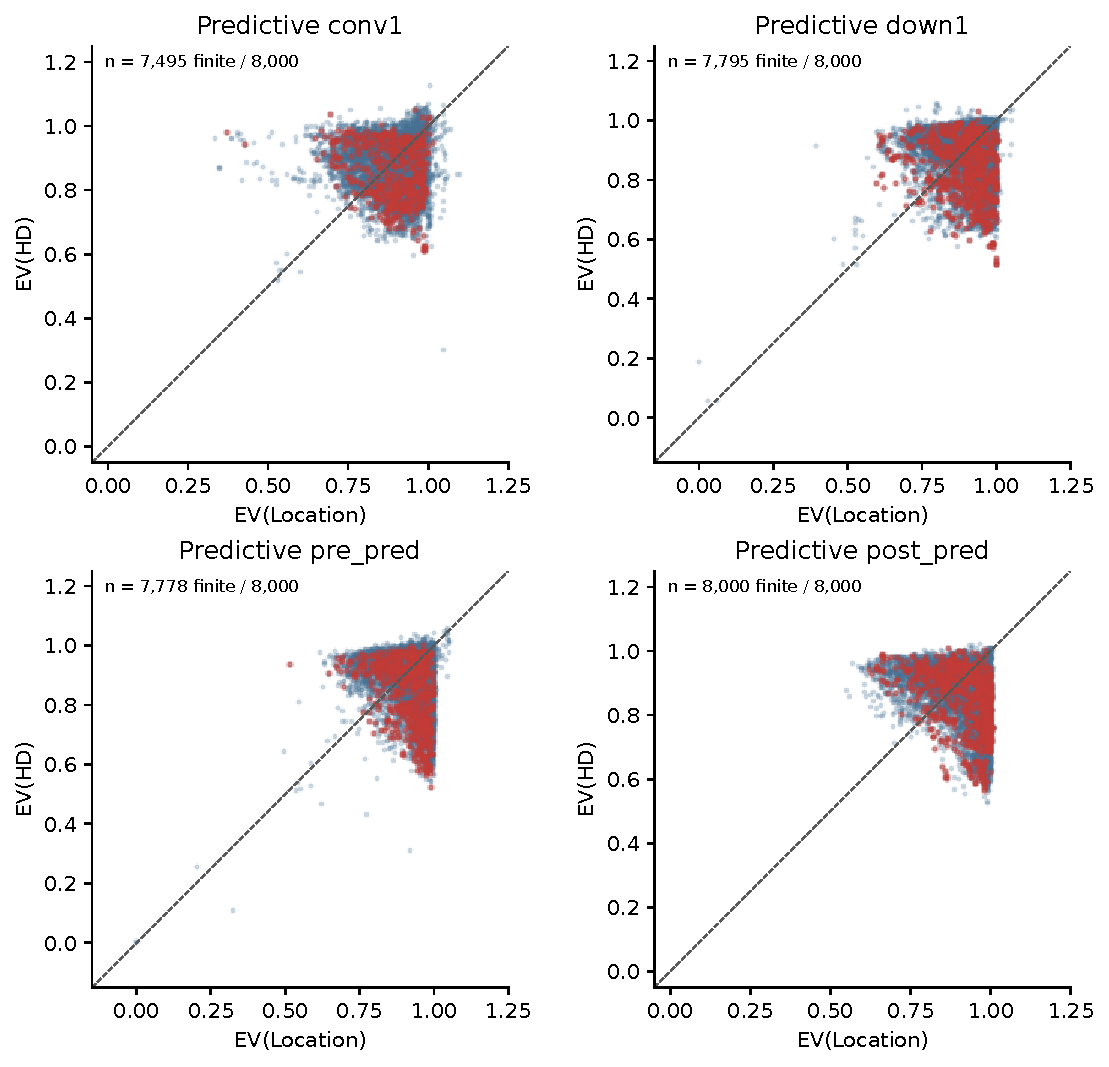
\includegraphics[width=.86\textwidth]{final_figures/pred_all_layers.pdf}
\caption{\textbf{Joint location and HD dependence across predictive-model layers.} Scores and finite denominators for the four analyzed layers of the causal-normalization checkpoint. Red points are exclusive place-classified units; all sampled units contribute to the corresponding classification summaries.}
\label{fig:si_pred_ev}
\end{figure}

\begin{figure}[htbp]
\centering
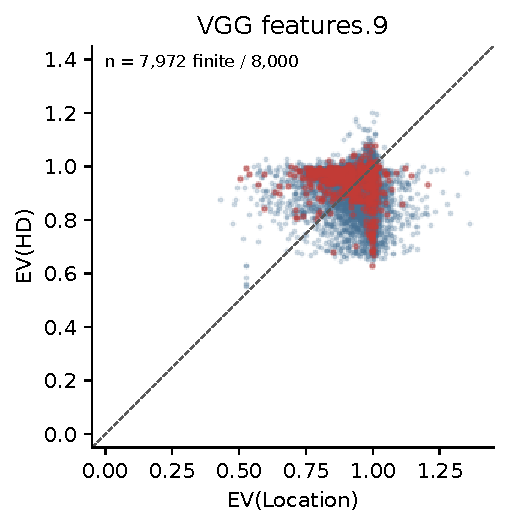
\includegraphics[width=.44\textwidth]{final_figures/vgg16_features.9_ev.pdf}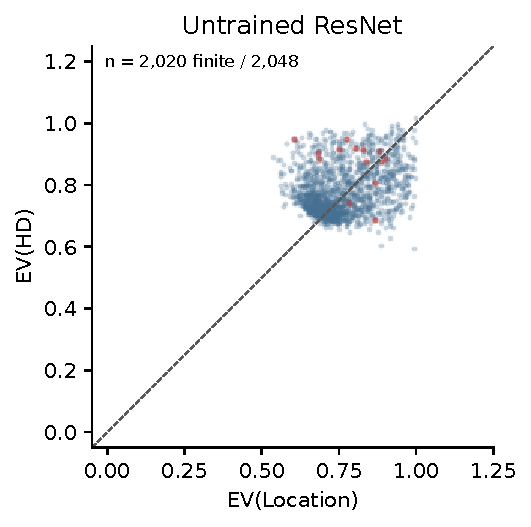
\includegraphics[width=.44\textwidth]{final_figures/resnet50_untrained_avgpool_ev.pdf}
\caption{\textbf{Other CNNs evaluated on the same panorama bank.} Left: ImageNet-pretrained VGG-16 features.9. Right: the fixed randomly initialized ResNet-50 avgpool layer. Red points indicate exclusive place classifications. Both location and HD are represented; the size and balance of the scores depend on architecture and training.}
\label{fig:si_cnn_ev}
\end{figure}

\subsection*{Scattered 3-D location$\times$HD firing fields in the CNN}

For example ResNet-50 units that pass the 2-D place cell classification, we plot the full 3-D rate map over 2-D location and head direction. These units respond to particular combinations of location and head direction, producing fragmented fields across head-direction slices. The population analysis quantifies their greater HD dependence relative to CA1 neurons (Fig.~\ref{fig:PlaceCell}). This is the CNN counterpart of the joint tuning shown for the predictive coding network in Fig.~\ref{fig:pred}.

\begin{figure}[p]
\centering
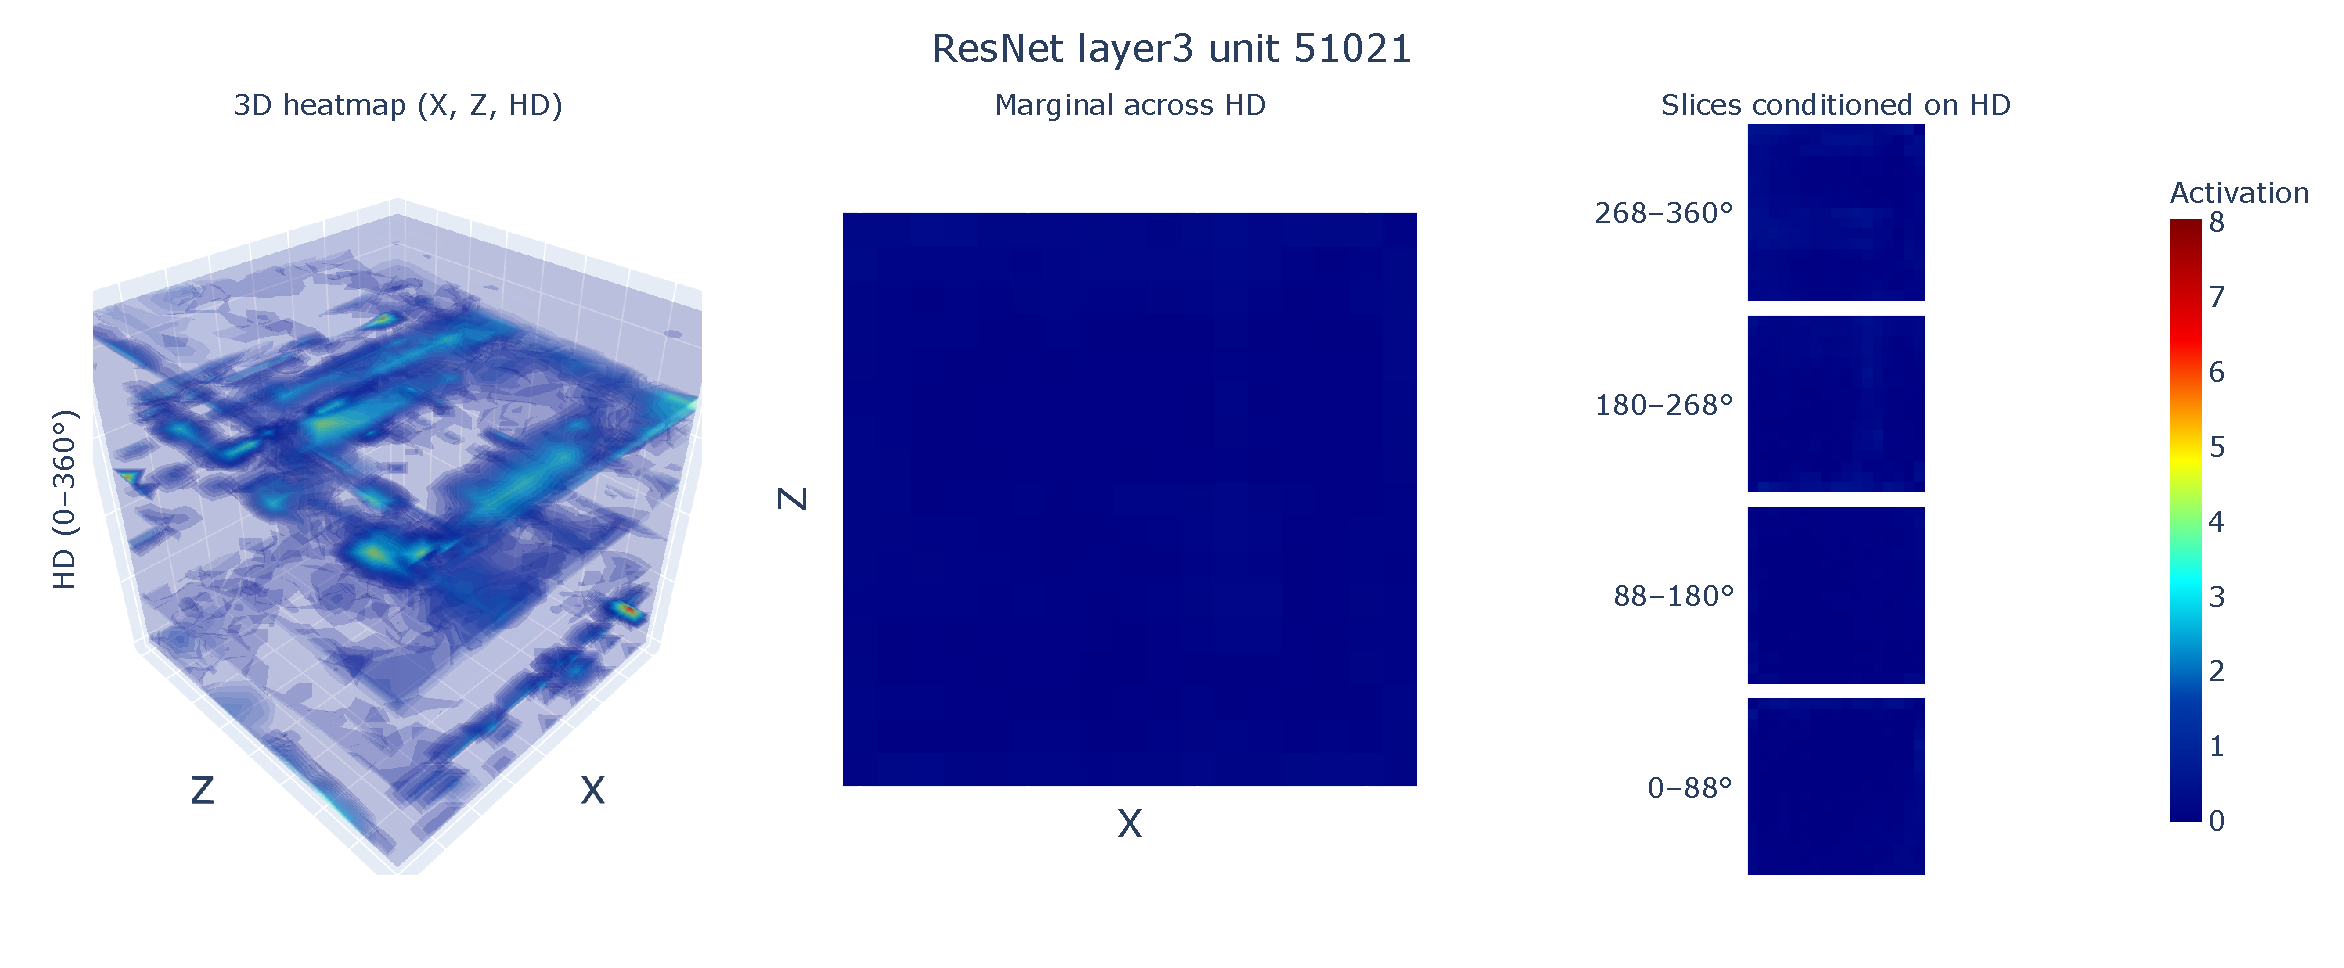
\includegraphics[width=.86\textwidth]{final_figures/resnet50_layer3_example.pdf}\\
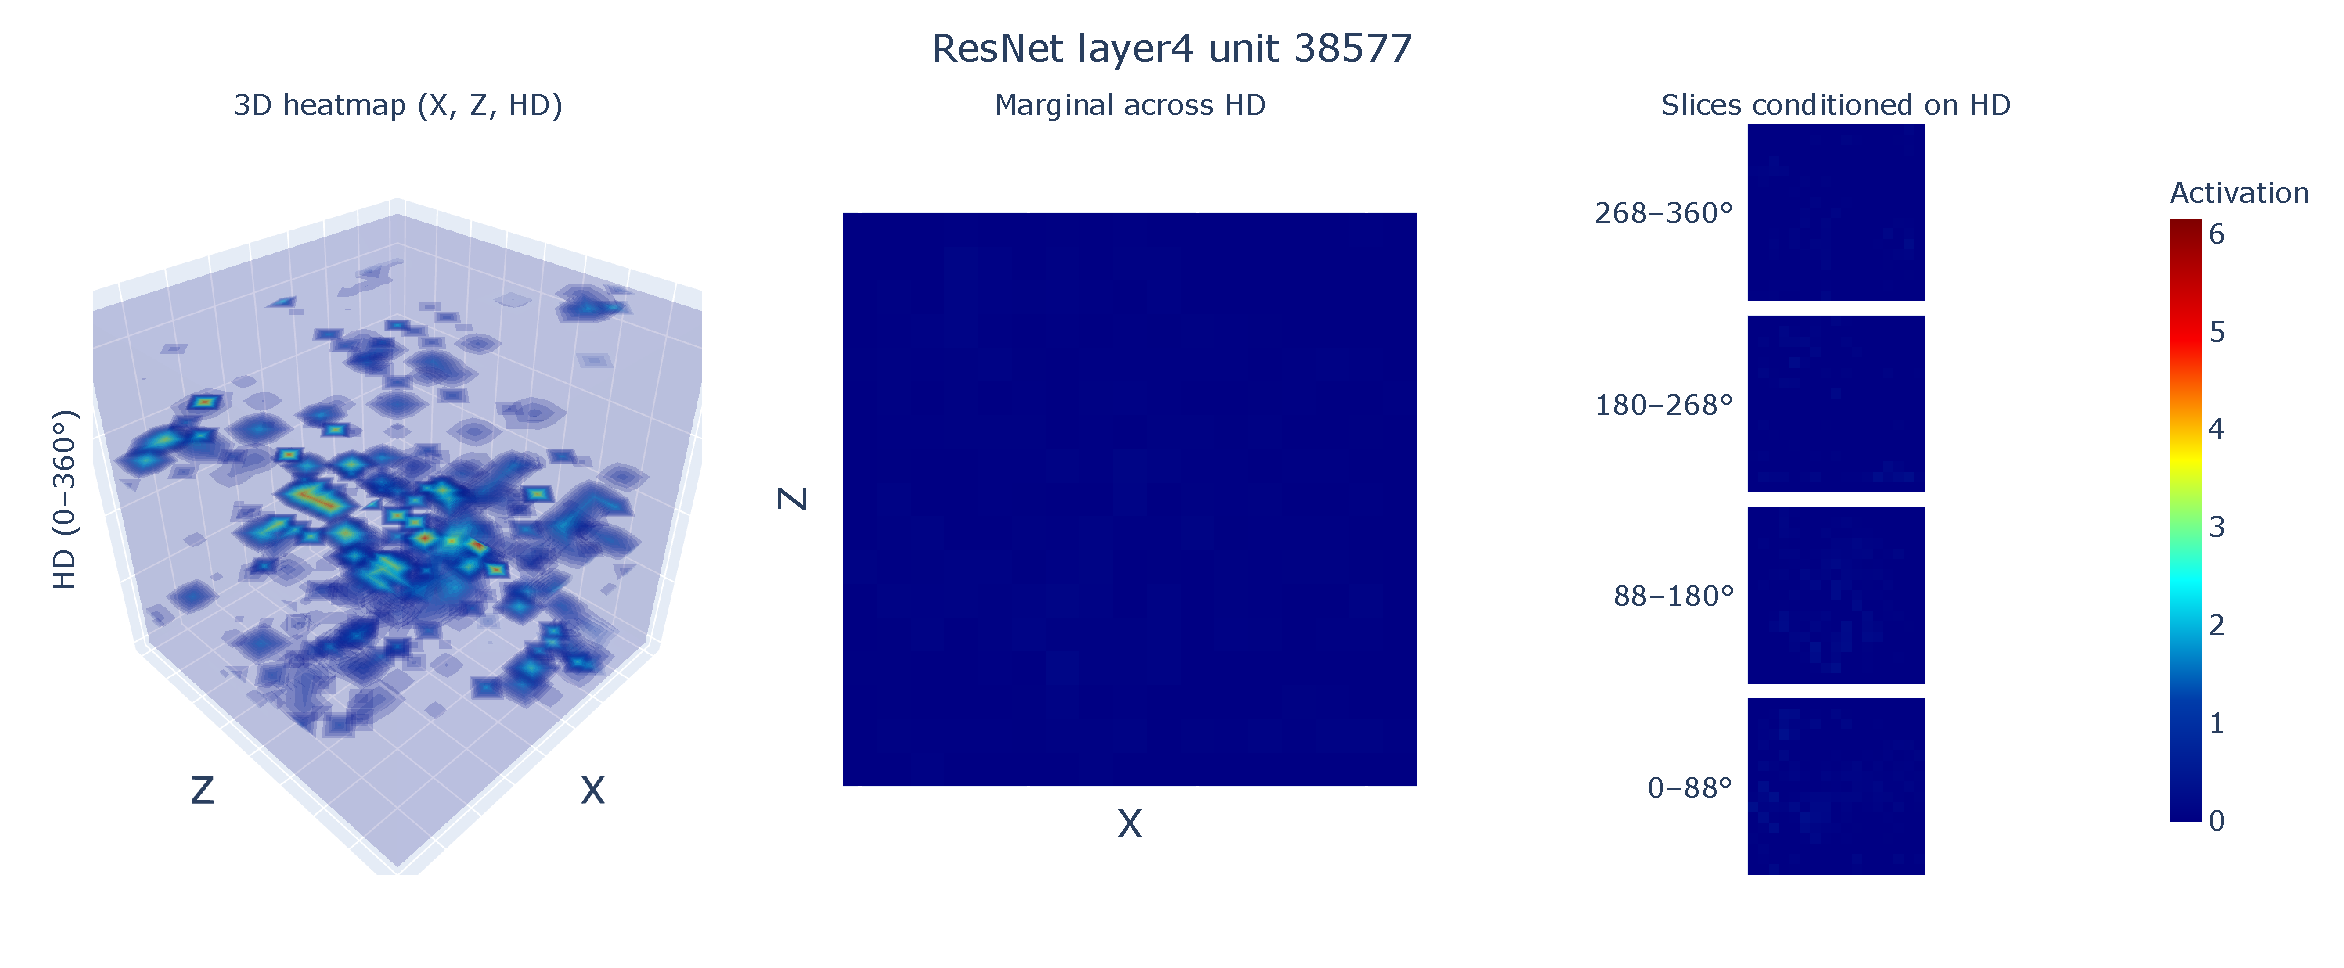
\includegraphics[width=.86\textwidth]{final_figures/resnet50_layer4_example.pdf}
\caption{\textbf{Joint maps of identified place-classified CNN units.} One randomly selected exclusive place-classified unit from each of ResNet-50 layer3 and layer4. Joint volume, mean map, and HD-sector maps use common limits within each unit. Unit IDs are recorded in the figure and reproduction metadata. Location fields change across HD sectors.}
\label{fig:si_scattered_maps}
\end{figure}

\subsection*{Sampling sensitivity of the split-half estimator}

On an axis to which the neuron is invariant, the true $\mathrm{EV}$ is 0, but the estimate can be elevated by sampling noise; $1-\langle C_{ii}\rangle_i$ provides a reliability-based reference, because identical tuning curves estimated from two finite halves of the data correlate imperfectly. The number of samples per bin sets the reliability $\langle C_{ii}\rangle_i$ and therefore this reference. Fig.~\ref{fig:si_floor} shows this reference for the $\theta=0\degree$ simulation of Fig.~\ref{fig:estimation} as a function of the number of samples at $15\times15$ bins. The bin-count sweep reported here is an additional numerical sensitivity analysis. With about 4 or more samples per bin, the reference is at most $0.05$ and $\mathrm{EV}(y)$ is close to it ($15\times15$ bins at $N=1{,}000$: $\mathrm{EV}(y)=0.054$, reference $0.052$). With 2 samples per bin or fewer, $\mathrm{EV}(y)$ exceeds the reference, and the reliability-normalized contribution no longer returns 0: at 30 bins per axis and $N=1{,}000$ (1.1 samples per bin), $\mathrm{EV}(y)=0.29$ with a reference of $0.14$; at $15\times15$ bins and $N=250$, $\mathrm{EV}(y)=0.35$ with a reference of $0.23$. The tuned axis is recovered in every condition ($\mathrm{EV}(x)$ between $0.99$ and $1.01$). We therefore report this reference together with $\mathrm{EV}$ for each dataset.

\begin{figure}[h!]
    \centering
    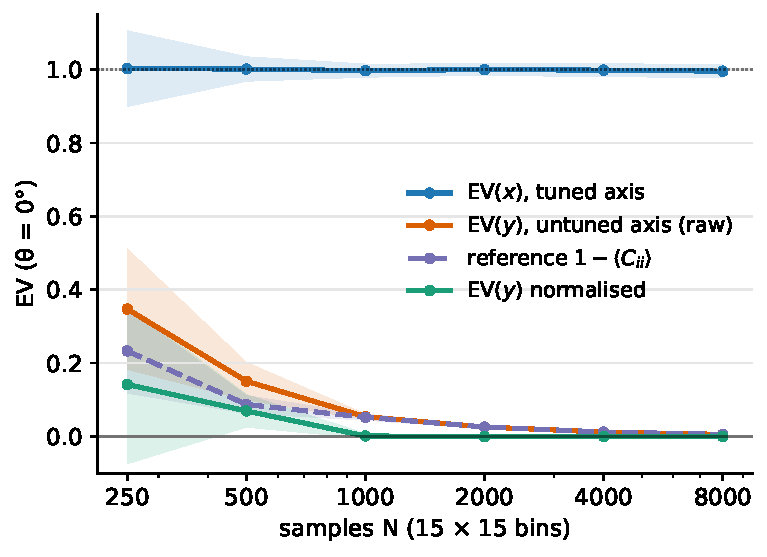
\includegraphics[width=0.65\textwidth]{final_figures/noise_floor_samples.pdf}
    \caption{\textbf{Sampling sensitivity of the split-half estimator.} Simulated neuron tuned to $x$ only ($\theta=0\degree$), so the true $\mathrm{EV}(y)=0$ and $\mathrm{EV}(x)=1$. Lines are means and shaded bands $\pm1$~s.d. over 100 simulated data sets. Varying the number of samples at $15\times15$ bins. Blue: $\mathrm{EV}(x)$ on the tuned axis. Orange: $\mathrm{EV}(y)=1-\langle C_{ij}\rangle_{i\neq j}$ on the untuned axis. Dashed purple: the noise reference $1-\langle C_{ii}\rangle_i$. Green: reliability-normalized $\mathrm{EV}_{\mathrm{norm}}(y)$. The untuned-axis estimate is close to the noise reference down to about 4 samples per bin; with sparser sampling it exceeds the reference. The tuned axis is recovered in every condition.}
    \label{fig:si_floor}
\end{figure}


\clearpage
\begin{figure}[htbp]
\centering
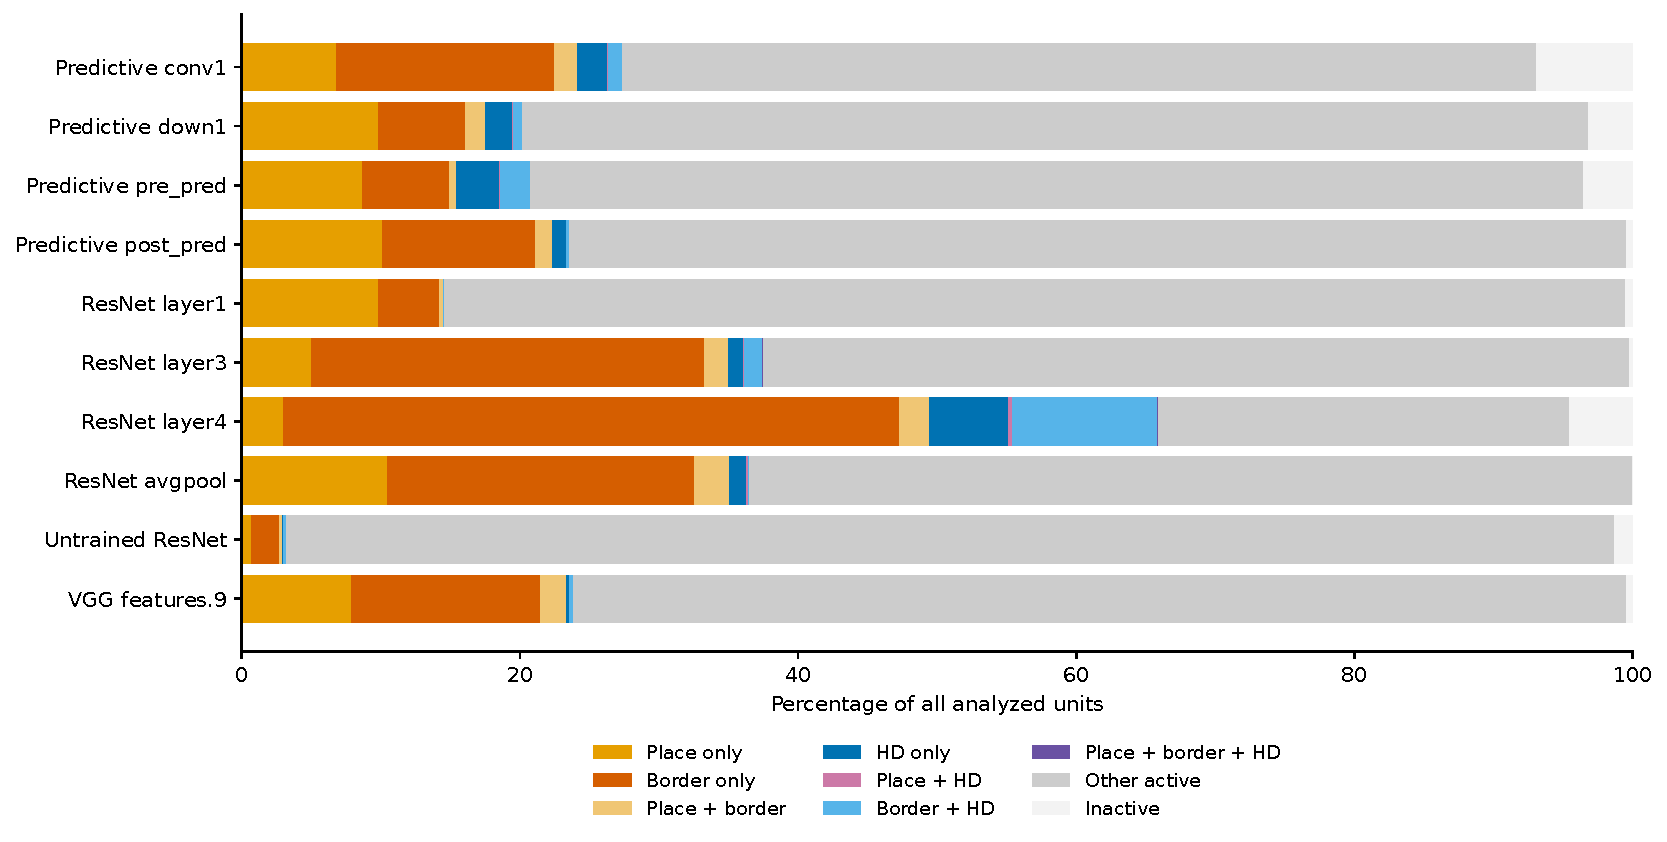
\includegraphics[width=.98\textwidth]{final_figures/detailed_classes.pdf}
\caption{\textbf{Detailed classification retains all place, border, and HD intersections.} Percentages use all sampled units, including inactive units. The main pies combine the place/border union into location selectivity without changing any classification or the exclusive-place subset.}
\label{fig:si_classes}
\end{figure}

\subsection*{Sensitivity to sampling and interpolation}
The primary biological contrast persists on native location$\times$HD grids: location exceeds HD in $74.1\%$ of finite CA1 estimates, and HD exceeds location in $82.5\%$ of HD-cell estimates. With finer spike bins, the CA1 preference remains $83.3\%$. In the finer $90\times90$ HD$\times$MD grid at zero lag, $1{,}139$ of $1{,}489$ cells have finite estimates on both axes; $92.8\%$ favor HD (median scores $0.97$ for HD and $0.52$ for MD). The $36\times36$ primary grid retains all cells, with corresponding medians $1.00$ and $0.21$. One- and three-sample MD shifts preserve the coarse-grid preference in $99.9\%$ of cells. These checks support the direction of the population contrasts while showing that the numerical magnitude of secondary-variable dependence is sensitive to support and binning.

\end{document}
